\documentclass[a4paper, 11pt]{article}
\usepackage{amsfonts}
\usepackage{epsfig}
\usepackage[italian]{babel}

\hyphenpenalty=10000
\tolerance=1000

%\usepackage[a4paper,margin=2cm]{geometry}
\usepackage[T1]{fontenc}
\usepackage{color}
\usepackage{alltt}
\usepackage{times}
\newcommand{\scitea}[1]{\noindent{\ttfamily{\textcolor[rgb]{0.0, 0.0, 0.0}{#1}}}}
\newcommand{\sciteb}[1]{\noindent{\ttfamily{\textcolor[rgb]{0.0, 0.5, 0.0}{#1}}}}
\newcommand{\scitec}[1]{\noindent{\ttfamily{\textcolor[rgb]{0.0, 0.5, 0.0}{#1}}}}
\newcommand{\sciteg}[1]{\noindent{\ttfamily{\textcolor[rgb]{0.5, 0.0, 0.5}{#1}}}}
\newcommand{\scitee}[1]{\noindent{\ttfamily{\textcolor[rgb]{0.0, 0.5, 0.5}{#1}}}}
\newcommand{\scitef}[1]{\noindent{\ttfamily{\textbf{\textcolor[rgb]{0.0, 0.0, 0.5}{#1}}}}}
\newcommand{\scitej}[1]{\noindent{\ttfamily{\textcolor[rgb]{0.5, 0.5, 0.0}{#1}}}}
\newcommand{\scitek}[1]{\noindent{\ttfamily{\textcolor[rgb]{0.0, 0.0, 0.0}{#1}}}}
\newcommand{\scitel}[1]{\noindent{\ttfamily{\textcolor[rgb]{0.0, 0.0, 0.0}{#1}}}}
\newcommand{\sciteib}[1]{\noindent{\ttfamily{\textcolor[rgb]{0.0, 0.0, 0.0}{#1}}}}

\newcommand{\code}[1]{\scriptsize{\texttt{#1}}\normalsize}


\begin{document}

\title{Implementazione di un compilatore per linguaggio Object Oriented}
\author{Lorenzo Dematt\'e}

\maketitle

\vspace{\stretch{1}}
\begin{abstract}
In questo documento, parte del mio esame di ``Linguaggi Formali e Compilatori'' presso l'universit\`a degli Studi di Trento, presento un compilatore per un linguaggio Object Oriented C++ - like, SMC, e le particolarit\`a, le caratteristiche e le difficolt\`a riscontrate durante la progettazione e l'implementazione dello stesso.
\end{abstract}
\vspace{\stretch{5}}
\pagebreak

\section{Il linguaggio SMC}

Il linguaggio SMC \`e un linguaggio Object Oriented ispirato al C++. Ovviamente il linguaggio \`e molto semplificato per ragioni di complessit\`a; tuttavia le caratteristiche pi\`u importanti di un linguaggio orientato agli oggetti sono presenti in SMC, e le maggiori problematiche che si riscontrano nella progettazione e nella realizzazione del compilatore per tale linguaggio sono state affrontate e risolte. In particolare, le seguenti caratteristiche sono supportate dal linguaggio:

\begin{itemize}
\item ereditariet\`a;
\item incapsulamento;
\item gestione della memoria dinamica;
\item passaggio di oggetti come parametri a funzioni;
\item polimorfismo attraverso funzioni virtuali;
\item corretta gestione dello scope per le variabili membro;
\item overloading.
\end{itemize}

Inoltre, per quanto riguarda la parte imperativa del linguaggio, sono state implementate le seguenti caratteristiche:

\begin{itemize}
\item passaggio di parametri per valore / per riferimento;
\item chiamate a funzione \emph{native}, cio\`e funzioni di libreria implementate dalla VM (si veda \cite{Fubi});
\item dichiarazione di variabili alla C++ (ovvero non solo all'inizio di un blocco, ma ovunque occorra).
\end{itemize}

Il compilatore poi \`e stato predisposto, mediante un design opportuno, per supportare e implementare agevolmente altre caratteristiche del linguaggio attualmente non previste. Tra queste:

\begin{itemize}
\item variabili e riferimenti \textbf{const};
\item namespace;
\item variabili di classe (\textbf{static}), variabili statiche;
\item ereditariet\`a multipla;
\item interfacce.
\end{itemize}

Sono stati implementati ma non approfonditamente testati gli \emph{array}; tale costrutto \`e da ritenersi sperimentale.

Per esempi di programmi scritti in SMC che implementano le caratteristiche sopra citate, si rimanda all'appendice.

\section{La struttura del compilatore}

Il compilatore \`e stato implementato in C++ secondo il modello a oggetti, seguendo un design ormai consolidato tra i compilatori, che prevede la distinzione tra front-end e back-end.
Il front-end, costituito da parser, scanner, e symbol table, si occupa della costruzione di un parse tree, che viene poi usato dal back-end per produrre codice oggetto. In particolare il back-end \`e a sua volta diviso in due parti: la prima prende come input il parse-tree e genera il corrispondente codice IL (Intermediate Language, codice intermedio), la seconda prende come input la Symbol Table e il codice IL per generare l'assembly vero e proprio. Questa ulteriore suddivisione consente, se in futuro si vorr\`a implementare questa caratteristica, di costruire agevolmente un compilatore per linguaggio target differente. E' sufficiente sostituire la parte che da codice IL e Symbol Table genera l'assembly.

\begin{figure}[ht]
\centering
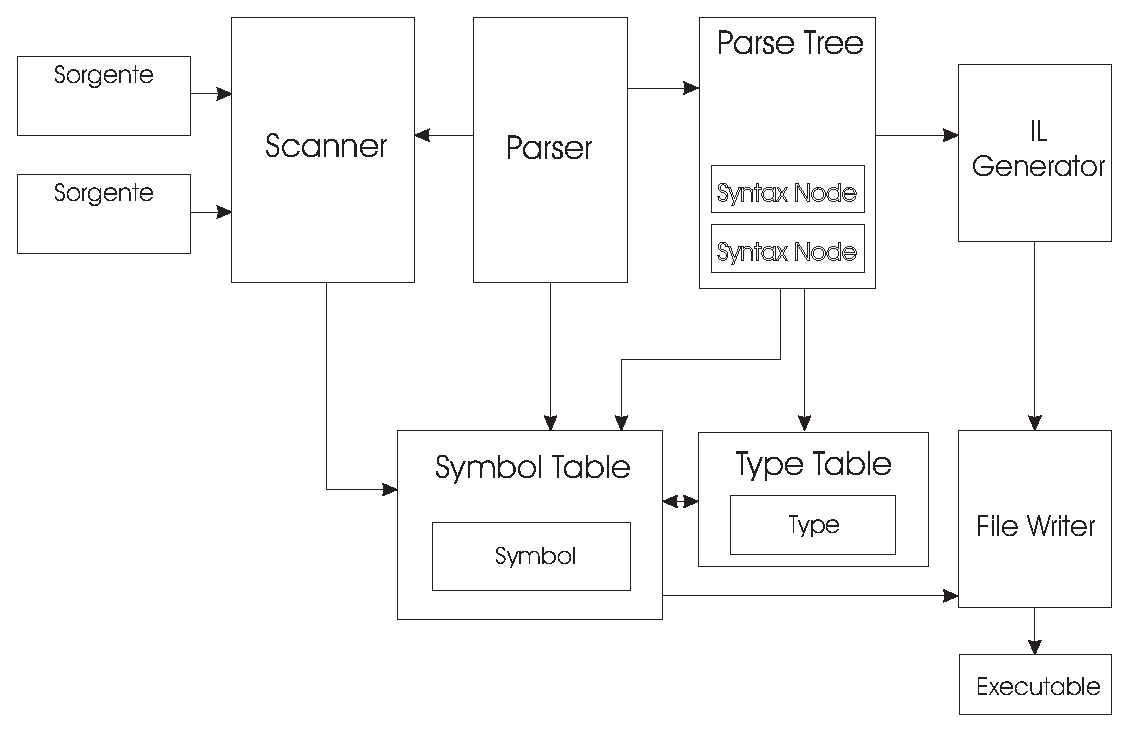
\includegraphics[width=0.8\textwidth]{compiler.eps}
\caption{La struttura a moduli del compilatore}
\label{fig:compiler}
\end{figure}

Di seguito sono illustate in maggiore dettaglio i pi\`u rilevanti di questi moduli.

\subsection{Symbol Table e Type Table}

In un linguaggio ad oggetti uno dei fattori pi\`u complessi \`e la gestione dello scope e della ricerca dei nomi nello namespace corrente. Una stessa variabile o funzione pu\`o essere definita pi\`u volte, ma la ricerca nello scope deve sempre dare il binding corretto.
Come esempio, si consideri il seguente blocco di codice:

%esempio2.cpp

\noindent
\scriptsize{
\scitea{} \\
\scitef{int}
\scitea{ }
\scitel{j}
\scitek{;}
\scitea{} \\
\scitea{} \\
\scitef{class}
\scitea{ }
\scitel{pippo}
\scitea{} \\
\scitek{\{}
\scitea{} \\
\scitef{public}
\scitek{:}
\scitea{} \\
\scitea{{\hspace*{1em}} } \\
\scitea{{\hspace*{1em}} }
\scitef{int}
\scitea{ }
\scitel{i}
\scitek{;}
\scitea{} \\
\scitea{{\hspace*{1em}} }
\scitef{int}
\scitea{ }
\scitel{j}
\scitek{;}
\scitea{} \\
\scitea{{\hspace*{1em}} } \\
\scitea{{\hspace*{1em}} }
\scitef{int}
\scitea{ }
\scitel{f}
\scitek{(}
\scitef{int}
\scitea{ }
\scitel{i}
\scitek{)}
\scitea{} \\
\scitea{{\hspace*{1em}} }
\scitek{\{}
\scitea{} \\
\scitea{{\hspace*{1em}}{\hspace*{1em}}{\hspace*{1em}} }
\scitef{return}
\scitea{ }
\scitel{i}
\scitea{ }
\scitek{*}
\scitea{ }
\scitel{j}
\scitek{;}
\scitea{ }
\scitec{//i is the parameter, j is member} \\
\scitea{{\hspace*{1em}} }
\scitek{\}}
\scitea{{\hspace*{1em}} } \\
\scitek{\};}
\scitea{} \\
\scitea{}
} %end tiny
\normalfont
\normalsize

Nella funzione \textbf{f} la variabile \textbf{i} deve essere legata al parametro e la variabile \textbf{j} alla variabile membro della classe pippo. 
Un modo efficiente per la ricerca e la risoluzione del binding di variabili \`e ottenibile ricorrendo a una Symbol Table che raccolga le informazioni su simboli e sulle definizioni dei tipi in modo gerarchico. Di seguito sono presentate parti delle due strutture che raccolgono tali informazioni: la classe \emph{SymDef} e la classe \emph{TypeRec}

\noindent
\scriptsize{
\scitea{} \\
\scitef{class}
\scitea{ }
\scitel{SymDef}
\scitea{} \\
\scitek{\{}
\scitea{} \\
\scitef{public}
\scitek{:}
\scitea{} \\
\scitea{{\hspace*{1em}} }
\scitec{//the name of the symbol} \\
\scitea{{\hspace*{1em}} }
\scitel{std}
\scitek{::}
\scitel{string}
\scitea{ }
\scitel{name}
\scitek{;}
\scitea{} \\
\scitea{} \\
\scitea{{\hspace*{1em}} }
\scitec{//the type of the symbol} \\
\scitea{{\hspace*{1em}} }
\scitel{TypePtr}
\scitea{ }
\scitel{type}
\scitek{;}
\scitea{} \\
\scitea{} \\
\scitea{{\hspace*{1em}} }
\scitec{//the owner of this symbol (scope)} \\
\scitea{{\hspace*{1em}} }
\scitel{SymPtr}
\scitea{ }
\scitel{parent}
\scitek{;}
\scitea{} \\
\scitea{} \\
\scitea{{\hspace*{1em}} }
\scitec{//symbol kind (class, variable, function...)} \\
\scitea{{\hspace*{1em}} }
\scitel{SYMBOL\_KIND}
\scitea{ }
\scitel{symKind}
\scitek{;}
\scitea{} \\
\scitea{} \\
\scitea{{\hspace*{1em}} }
\scitec{//the list of "sons" (symbols declared in this scope)} \\
\scitea{{\hspace*{1em}} }
\scitel{std}
\scitek{::}
\scitel{list}
\scitek{$<$}
\scitel{SymPtr}
\scitek{$>$}
\scitea{ }
\scitel{declList}
\scitek{;}
\scitea{} \\
\scitea{} \\
\scitea{{\hspace*{1em}} }
\scitec{//CLASS MEMBERS} \\
\scitea{{\hspace*{1em}} }
\scitec{//NAMESPACE MEMBERS} \\
\scitea{{\hspace*{1em}} }
\scitec{//SCOPEBLOCK MEMBERS} \\
\scitea{{\hspace*{1em}} }
\scitec{//FUNCTION MEMBERS} \\
\scitea{{\hspace*{1em}} }
\scitec{//VARIABLE{\hspace*{1em}} MEMBERS} \\
\scitea{{\hspace*{1em}} }
\scitec{//TYPEDEF MEMBERS} \\
\scitek{\};}
\scitea{} \\
\scitea{} \\
\scitea{} \\
\scitea{}
} %end tiny
\normalfont
\normalsize


\noindent
\scriptsize{
\scitef{class}
\scitea{ }
\scitel{TypeDef}
\scitea{} \\
\scitek{\{}
\scitea{} \\
\scitef{public}
\scitek{:}
\scitea{} \\
\scitea{{\hspace*{1em}} }
\scitel{TYPE\_TYPE}
\scitea{ }
\scitel{typeID}
\scitek{;}
\scitea{} \\
\scitea{} \\
\scitea{{\hspace*{1em}} }
\scitec{//types used by this one} \\
\scitea{{\hspace*{1em}} }
\scitel{std}
\scitek{::}
\scitel{deque}
\scitek{$<$}
\scitel{TypePtr}
\scitek{$>$}
\scitea{ }
\scitel{typeList}
\scitek{;}
\scitea{} \\
\scitea{} \\
\scitea{{\hspace*{1em}} }
\scitec{//type modifiers} \\
\scitea{{\hspace*{1em}} }
\scitef{bool}
\scitea{ }
\scitel{isConst}
\scitek{;}
\scitea{} \\
\scitea{{\hspace*{1em}} }
\scitef{bool}
\scitea{ }
\scitel{isReference}
\scitek{;}
\scitea{} \\
\scitea{{\hspace*{1em}} }
\scitef{bool}
\scitea{ }
\scitel{isPointer}
\scitek{;}
\scitea{} \\
\scitea{} \\
\scitea{{\hspace*{1em}} }
\scitef{int}
\scitea{ }
\scitel{arraySize}
\scitek{;}
\scitea{} \\
\scitea{{\hspace*{1em}} }
\scitel{std}
\scitek{::}
\scitel{string}
\scitea{ }
\scitel{name}
\scitek{;}
\scitea{} \\
\scitea{{\hspace*{1em}} }
\scitel{SymPtr}
\scitea{ }
\scitel{symbol}
\scitek{;}
\scitea{} \\
\scitek{\};}
} 
\normalfont
\normalsize


Come si pu\`o vedere dalla dichiarazione, la classe \emph{SymDef} rappresenta la definizione di un simbolo valido all'interno del programma da compilare. Ogni simbolo ha un puntatore al padre e contiene la lista dei simboli figli, ovvero la lista dei nomi definiti direttamente all'interno del suo scope\footnote{I simboli definiti direttamente all'interno dello scope variano a seconda del simbolo padre: per una funzione sono i parametri e le variabili locali, per una classe sono variabili e funzioni membro, ecc..}.
Questo consente di creare una struttura ad albero che rappresenta direttamente la struttura gerarchica dei simboli e permette di ricercare un simbolo efficientemente.
All'interno di un oggetto SymDef vengono inoltre immagazzinate tutte le informazioni utili riguardanti il simbolo. Nell'implementazione, al posto del vari commenti, sono presenti i membri della class SymDef rilevanti rispettivamente quando la specie del simbolo \`e \code{class}, \code{namespace}, \code{function}, \code{variable}, ecc.
Questi campi contengono le informazioni pi\`u disparate, valide a seconda della specie del simbolo: per le variabili, ad esempio, se \`e parametro o membro di classe, per le funzioni se \`e virtuale e il suo eventuale indice all'interno della tabella delle funzioni virtuali, e cos\`{i} via.
\\
Strettamente collegata alla \emph{symbol table} e ai suoi record (gli oggetti SymDef) \`e la \emph{type table} con i suoi record (costituiti da oggetti TypeRec). Analogamente alla precedente, tale tabella ha una struttura gerarchica rappresentata tramite un albero. I due alberi sono correlati tra di loro: ogni SymDef contiene un puntatore a un TypeRec che rappresenta il tipo del simbolo. Inoltre per quanto riguarda i tipi di dato definiti dall'utente (nel nostro caso, le classi) il TypeRec contiene un puntatore al simbolo che definisce l'UDT\footnote{UDT: User Data Type, tipo di dato definito dall'utente}.
\begin{figure}[ht]
\centering
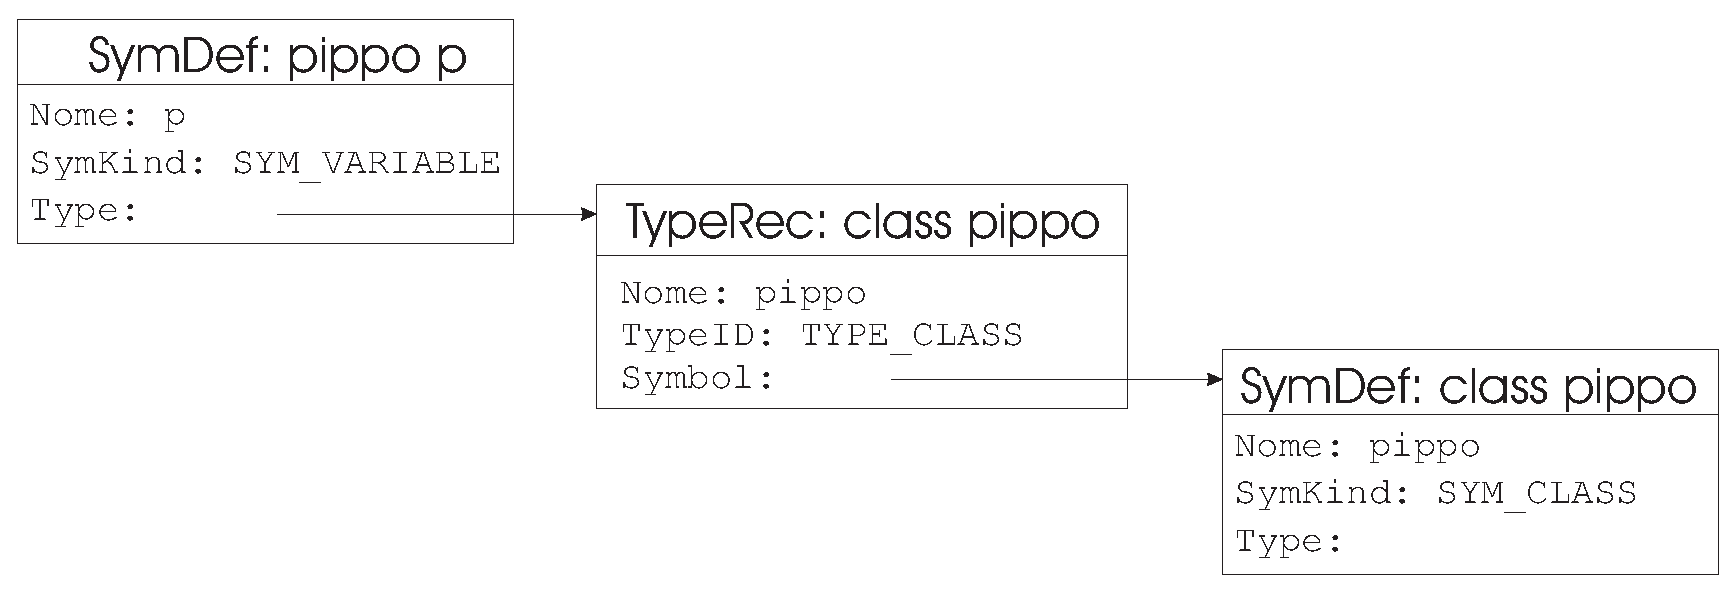
\includegraphics[width=0.85\textwidth]{esempio1.eps}
\caption{Esempio di relazione tra gli elementi della symbol table e della type table}
\label{fig:esempio1}
\end{figure}


\pagebreak
\noindent
Per esempio, il codice seguente:

%esempio1.cpp
\noindent
\scriptsize{
\scitef{class}
\scitea{ }
\scitel{pippo}
\scitea{} \\
\scitek{\{}
\scitea{} \\
\scitef{public}
\scitek{:}
\scitea{} \\
\scitea{{\hspace*{1em}} }
\scitef{int}
\scitea{ }
\scitel{i}
\scitek{;}
\scitea{} \\
\scitek{\};}
\scitea{} \\
\scitea{} \\
\scitel{pippo}
\scitea{ }
\scitel{p}
\scitek{;}
\scitea{} \\
\scitea{}
}
\normalfont
\normalsize
\\
porta alla struttura in figura~\ref{fig:esempio1}

\pagebreak

\section{Il linguaggio assembly e la VM (Virtual Machine)}

Il compilatore SMC attualmente ha come linguaggio target un linguaggio assembly per una macchina virtuale costruita ad hoc. Questo consente di trattare in modo pi\`u semplice aspetti come funzioni virtuali, gestione della memoria dinamica, ecc. concentrandosi sulle funzionalit\`a. 

Il linguaggio assembly e la macchina virtuale sono stati pensati per lavorare insieme; le loro principali caratteristiche sono:
\begin{itemize}
\item unica forma per i dati, sia in memoria che su disco: gli operandi delle istruzioni, gli elementi dello Stack, i registri della macchina virtuale, le variabili membro degli oggetti sono tutti tipi di dato \code{struct Operand}

\begin{figure}[ht]
\centering
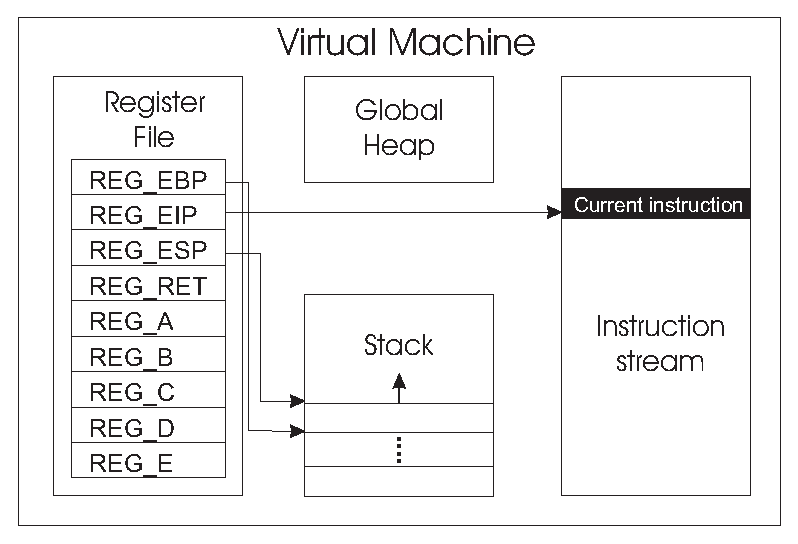
\includegraphics[width=0.75\textwidth]{vm.eps}
\caption{La Virtual Machine}
\label{fig:vm}
\end{figure}

\item
la macchina virtuale \`e costruita secondo lo schema in figura \ref{fig:vm}: ha 9 registri (4 riservati, 5 disponibili all'utente), uno spazio di memoria dinamico (heap), uno stack e una CPU virtuale che esegue il programma in input passo dopo passo, completando per ogni istruzione le seguenti fasi: decodifica dell'istruzione, reperimento degli operandi, esecuzione, memorizzazione del risultato.

\begin{figure}[ht]
\centering
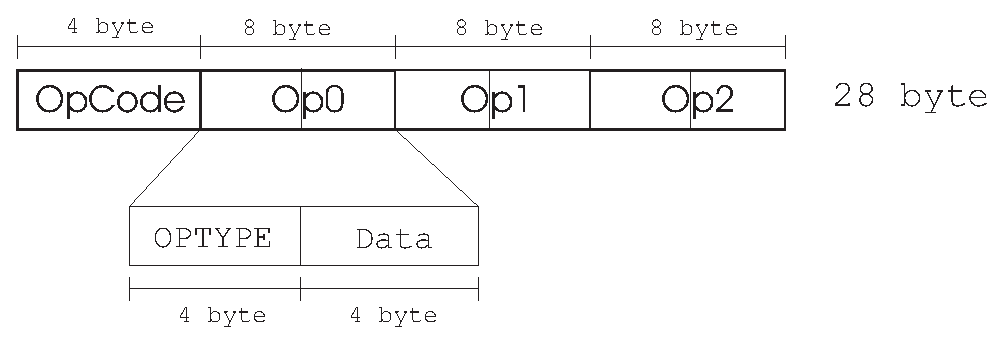
\includegraphics[width=0.75\textwidth]{instr.eps}
\caption{Struttura delle istruzioni e degli operandi}
\label{fig:instr}
\end{figure}

\item per ragioni di semplicit\`a, le istruzioni hanno lunghezza fissa e struttura a \emph{three operands}, come in figura \ref{fig:instr}



\end{itemize}

La struttura che consente di immagazzinare ogni dato all'interno del file eseguibile e nella memoria della VM \`e illustrata in figura \ref{fig:instr}.\\
Questa struttura, chiamata comunemente \emph{tagged union}, permette di memorizzare al suo interno tipi di dati diversi; il significato del dato contenuto \`e poi interpretato in maniera diversa a seconda del valore del tag.
Nella seguente tabella sono illustati i vari tipi di dati memorizzabili da una struttura \code{Operand}.
I vari tipi di Indirizzamento nella terza colonna sono illustrati in figura \ref{fig:operands}

\begin{figure}[ht]
\centering
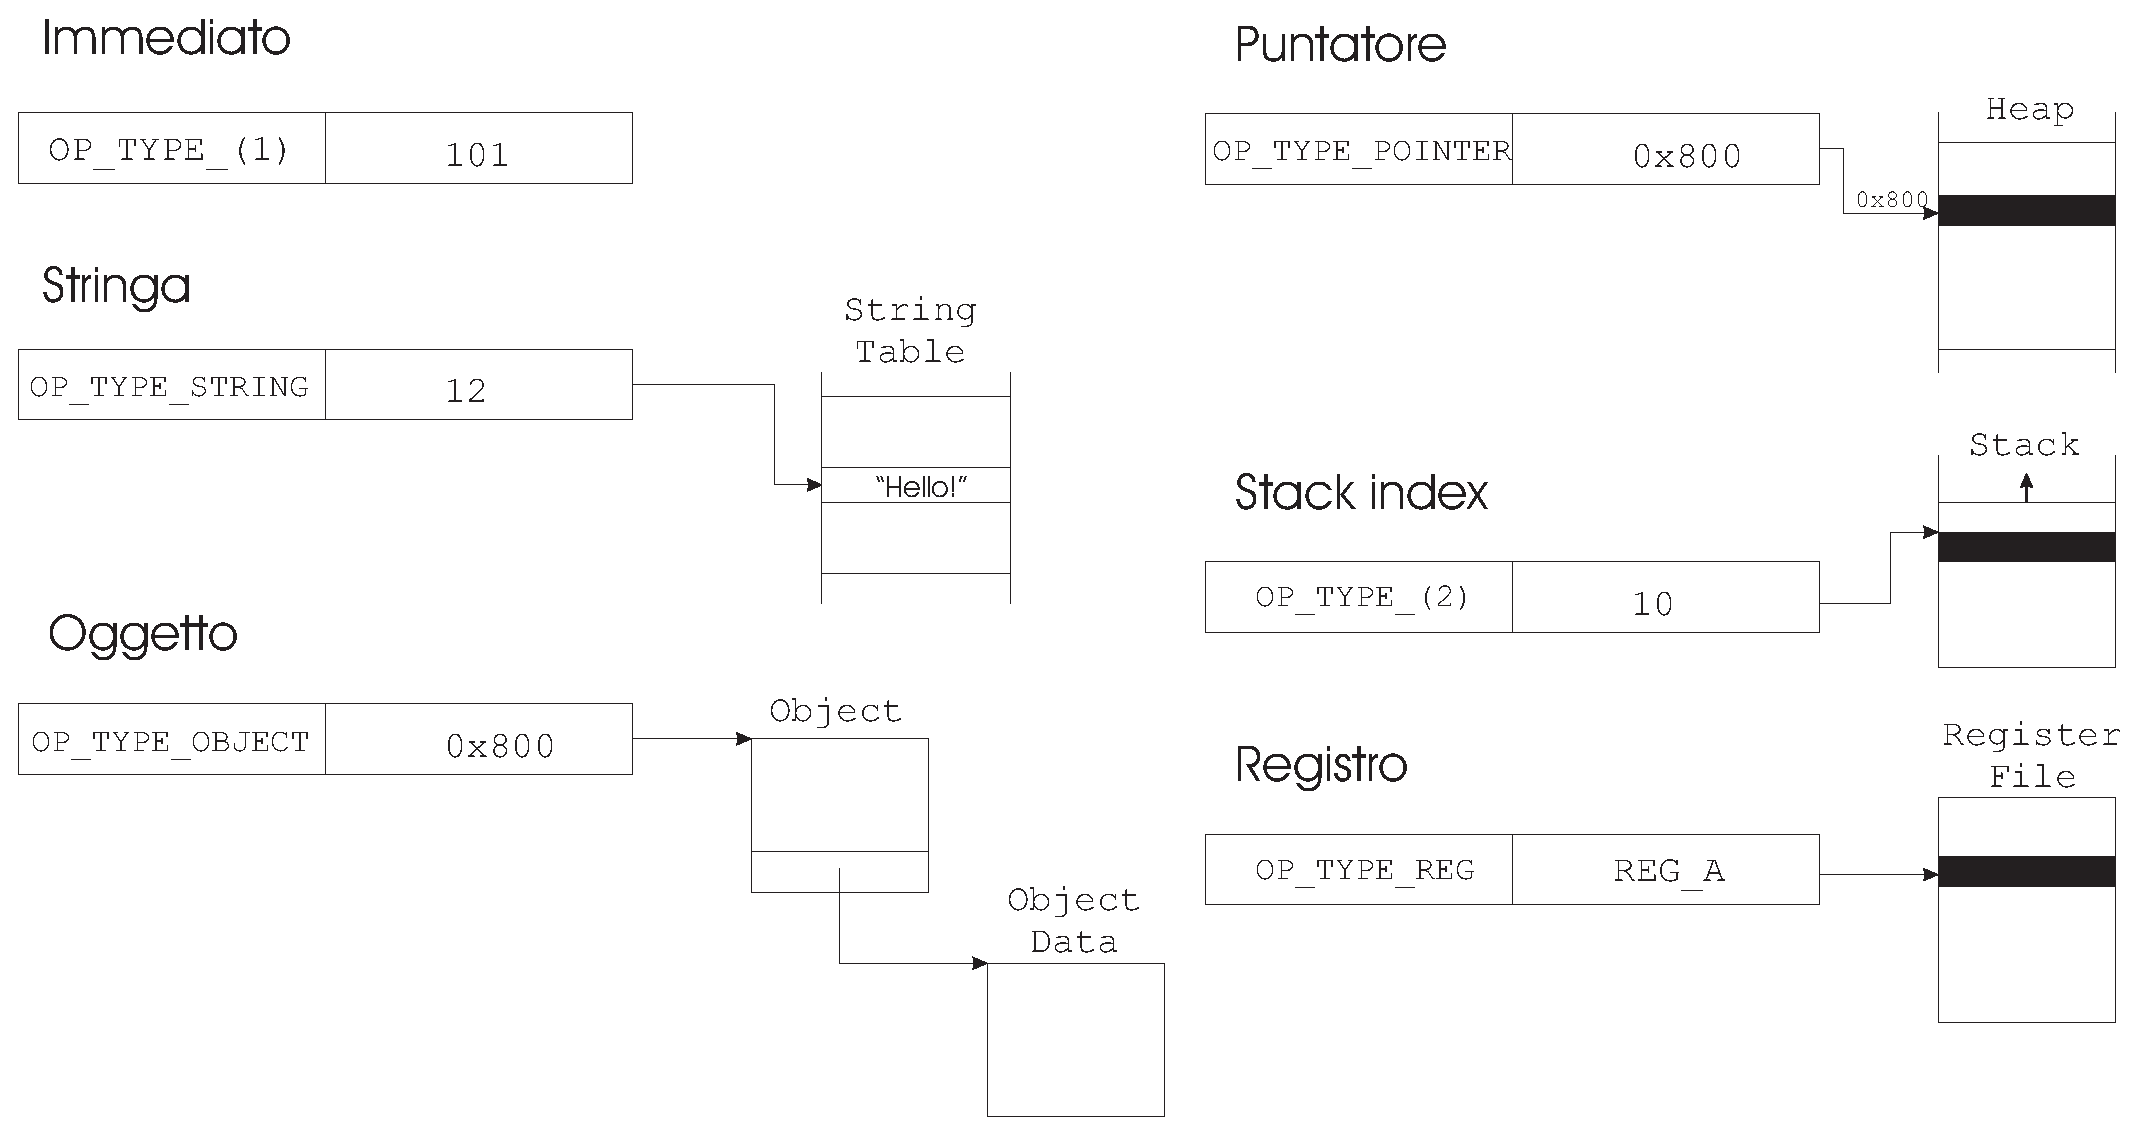
\includegraphics[width=\textwidth]{operands.eps}
\caption{I vari tipi di indirizzamento. Per quelli nella colonna di destra, in nero \`e evidenziato il dato (sempre \code{Operand}) su cui vengonono effettivamente svolte le operazioni. \code{OP\_TYPE\_(1)} sta per \code{INT, FLOAT, INSTR\_INDEX, FUNC, OBJECT\_TAG} e \code{TYPE\_TAG}; \code{OP\_TYPE\_(2)} sta per \code{ABS\_STACK\_INDEX} e \code{REL\_STACK\_INDEX}.}
\label{fig:operands}
\end{figure}

\begin{center}
\begin{tabular}{l|c|c}
\hline
\textbf{Tag} & \textbf{Tipo del dato} & \textbf{Indirizzamento}\\
\hline
  \code{OP\_TYPE\_INT} & integer (32-bit) & Immediato\\
  \code{OP\_TYPE\_FLOAT} & floating point (32-bit) & Immediato\\
   \code{OP\_TYPE\_STRING} & stringa & Stringa\\

   \code{OP\_TYPE\_ABS\_STACK\_INDEX} & integer (32-bit) & Stack index\\
   \code{OP\_TYPE\_REL\_STACK\_INDEX} & integer (32-bit) & Stack index\\

   \code{OP\_TYPE\_OBJECT} &  Object* & Oggetto\\
   \code{OP\_TYPE\_POINTER} & pointer & Puntatore\\
   \code{OP\_TYPE\_ARRAY} & ObjectArray* & Oggetto \\

   \code{OP\_TYPE\_INSTR\_INDEX} & integer (32-bit) & Immediato\\
   \code{OP\_TYPE\_FUNC} & integer (32-bit) & Immediato\\
   \code{OP\_TYPE\_REG} & integer (32-bit) & Registro\\

   \code{OP\_TYPE\_OBJECT\_TAG} & tag  & Immediato\\
   \code{OP\_TYPE\_TYPE\_TAG} & tag & Immediato\\
\hline
\end{tabular}
\end{center}

Le istruzioni assembly con la descrizione del loro significato e degli operandi sono presentate nella seguente tabella:



\begin{center}
\begin{tabular}{p{2.2 cm}|c|c|p{5.5 cm}}
\hline
\textbf{Istruzione} & \textbf{No. op} & \textbf{Tipo op} & \textbf{Descrizione}\\
\hline


\code{ADD, SUB, MUL, DIV, MOD} & 3 & \code{INT} & \footnotesize{Eseguono rispettivamente addizione, sottrazione, moltiplicazione, divisione, modulo tra gli operandi 1 e 2 e salvano il risulatato nell'operando 0. Esempio: \linebreak \code{ADD REG\_A REG\_B REG\_C}: \code{op[REG\_A] := op[REG\_B] + op[REG\_C]}}\\

\code{INC, DEC} & 1 & \code{INT} & \footnotesize{Incrementano o decrementano di un'unit\`a l'operando 0.}\\

\code{MOV} & 2 & any & \footnotesize{Recupera l'elemento nell'operando 1 e lo assegna al dato \emph{puntato} dall'operando 0. Esempio:} 
\linebreak \code{REG\_A = \{OP\_TYPE\_POINTER, 0x300\}} 
\linebreak \code{MOV REG\_A 10}: \code{heap[0x300] := 10} 
\linebreak \code{REG\_A} \footnotesize{resta invariato.}\\

\code{SET} & 2 & any & \footnotesize{Recupera l'elemento nell'operando 1 e lo assegna all'operando 0. Esempio:} \linebreak \code{REG\_A = \{OP\_TYPE\_POINTER, 0x300\}} \linebreak \code{SET REG\_A 10}: 
\linebreak \code{REG\_A = \{OP\_TYPE\_INT, 10\}} 
\linebreak \code{heap[0x300]}
\footnotesize{resta invariato.}\\

\code{PUSH} & 1 & any & \footnotesize{Mette il dato indicato nell'openado 0 sullo stack. Nel caso di un operando di tipo} \code{OBJECT} \footnotesize{incrementa il contatore di riferimenti.}\\

\code{POP} & 1 & any & \footnotesize{Prende il dato indicato in cima allo stack e lo muove nella locazione indicanta dall'openado 0, rimuovendolo dallo stack.}\\

\code{TOP} & 1 & any & \footnotesize{Mette il dato indicato in cima allo stack nell'openado 0. Lo stack rimane invariato.}\\

\code{AND, OR, XOR, LSH, RSH} & 3 & \code{INT} & \footnotesize{Eseguono rispettivamente le operazioni bit a bit di and, or inclusivo, or esclusivo, shift a sinistra e shift a destra tra gli operandi 1 e 2, salvando il risulatato nell'operando 0. }\\

\code{NEG} & 2 & \code{INT} & \footnotesize{Esegue la negazione bit a bit dell'operando 1 salvando il risulatato nell'opernado 0.}\\

\code{FADD, FSUB, FMUL, FDIV} & 3 & \code{FLOAT} & \footnotesize{Eseguono rispettivamente addizione, sottrazione, moltiplicazione e divisione tra gli operandi 1 e 2 e salvano il risulatato nell'operando 0.}\\

\code{FSQRT} & 3 & \code{FLOAT} & \footnotesize{Esegue l'estrazione di radice quadrata sul numero referenziato da op1 salvando il risulatato in op0.}\\

\hline
\end{tabular}
\end{center}

\begin{center}
\begin{tabular}{p{2.2 cm}|c|c|p{5.5 cm}}
\hline

\textbf{Istruzione} & \textbf{No. op} & \textbf{Tipo op} & \textbf{Descrizione}\\
\hline


\code{CALL} & 2 & \code{TAG, INT} & \footnotesize{Chiama la funzione con ordinale in op1 membro dell'oggetto con ID in op0.}\\
\code{VCALL} & 1 & \code{INT} & \footnotesize{Chiama la funzione virtuale con ordinale in op0 membro dell'oggetto corrente.}\\

\code{RET} & 1 & \code{INT} & \footnotesize{Ritorna dalla funzione. Il valore in op0 indica il numero di posizioni sullo stack da liberare.}\\

\code{I2F, F2I, STR2I, STR2F, I2STR, F2STR} & 2 & vari & \footnotesize{Istruzioni di conversione rispettivamente da (op1) a (op0):
\linebreak \code{ INT -> FLOAT }
\linebreak \code{ FLOAT -> INT }
\linebreak \code{ STRING -> INT }
\linebreak \code{ STRING -> FLOAT }
\linebreak \code{ INT -> STRING }
\linebreak \code{ FLOAT -> STRING }
}\\

\code{UCAST, DCAST} & 3 & \code{OBJECT, OBJECT, TAG} & \footnotesize{Upcast e downcast dell'oggetto in op1. Op2 contiene l'ID della classe target.} \code{DCAST} \footnotesize{pu\`o generare un'eccezione se il tipo non \`e corretto.}\\

\code{STORE} & 2 & \code{POINTER}, any & \footnotesize{Memorizza nella locazione di memoria puntata da op0 il dato referenziato da op1.}\\

\code{RELEASE} & 1 & \code{OBJECT} & \footnotesize{Rilascia un riferimento a un oggetto. Se il reference count per l'oggetto arriva a 0, questo viene cancellato.}\\

\code{PADD, PSUB} & 3 & \code{POINTER, POINTER, INT} & \footnotesize{Aggiunge o sottrae un offeset specificato in op2 dall'indirizzo di memoria in op1, memorizzando il risultato in op0. }\\
\code{LEA} & 2 & \code{POINTER}, vari & \footnotesize{Carica l'indirizzo di memoria di op1 in op0. Equivalente a \code{op0 = \&op1} }\\
\code{LEAA} & 2 & \code{POINTER, ARRAY, INT} & \footnotesize{Carica l'indirizzo di memoria dell'elemento dell'array in op1 con indice in op2 nell'operando referenziato in op0. Equivalente a \code{op0 = \&(op1[op2])} }\\

\code{NEW} & 2 & \code{OBJECT, TAG} & \footnotesize{Crea un nuovo oggetto del tipo specificato in op1.}\\
\code{NEWA} & 3 & \code{OBJECT, TAG, INT} & \footnotesize{Crea un array con elementi del tipo specificato in op1 e dimensione specificata in op2.}\\

\code{CLONE} & 2 & \code{OBJECT} & \footnotesize{Clona l'oggetto referenziato dall'operando 1. Un clone condivide l'area dati dell'oggetto, ma ha un diverso riferimento e, possibilmente, un diverso tipo.}\\

\code{HALT} & 0 &  & \footnotesize{Arresta la VM (ultima istruzione eseguita).}\\


\hline
\end{tabular}
\end{center}

\begin{center}
\begin{tabular}{p{2.2 cm}|c|c|p{5.5 cm}}
\hline
\textbf{Istruzione} & \textbf{No. op} & \textbf{Tipo op} & \textbf{Descrizione}\\
\hline


\code{JMP} & 1 & \code{INT} & \footnotesize{Salto incondizionato all'istruzione in op0.}\\
\code{JNEG JZ JNZ} & 2 & \code{INT or FLOAT}, \code{INT} & \footnotesize{Salto all'istruzione in op1 se $op0<0$, $op0=0$, $op0\neq 0$}\\
\code{JE, JNE, JLE, JGE, JL, JG} & 3 & \code{INT or FLOAT}, \code{INT or FLOAT}, \code{INT} & \footnotesize{ Salto all'istruzione in op2 se $op0 = op1$, $op0 \neq op1$, $op0 \leq op1$, $op0 \geq op1$, $op0 < op1$, $op0 > op1$, }\\

\hline
\end{tabular}
\end{center}

\section{Peculiarit\`a e difficolt\`a riscontrate}

Di seguito sono illustrati gli aspetti di design e di implementazione che distinguono 
un compilatore per un linguaggio imperativo da un compilatore per un linguaggio ad oggetti; 
inoltre sono discussi gli aspetti che si sono rivelati pi\`u problematici o pi\`u interessanti.

\subsection{TYPENAME vs. IDENTIFIER}

Facendo il parsing di qualsiasi linguaggio C/C++ like che permetta la definizione 
di tipi da parte dell'utente si presenta un interessante problema\cite{Ros91}. Anzitutto bisogna notare
che esistono due forme distinte di `identificatori' che possono essere letti dal lexer durante la fase di
analisi lessicale, identificati entrambi come simboli terminali nella mia grammatica.
Questi token terminali sono chiamati IDENTIFIER  e  TYPENAME; questa distinzione \`e 
necessaria a causa di un elemento fondamentale dei linguaggi C-like. 
Un lexeme di tipo TYPENAME si presenta come un identificatore standard, ma 
\`e definito nella symbol table come un tipo di dato dichiarato in precedenza 
(class, nel nostro caso, ma anche typedef, struct, enum). 
Tutti gli altri lexeme che compaiono come identificatori e che non sono keywords del
linguaggio sono tokenizzati come IDENTIFIER.
\\
Perch\'e questa distinzione \`e necessaria? Si consideri il codice seguente:
\\
\noindent
\scriptsize{
\scitef{class}
\scitea{ }
\scitel{A}
\scitek{;}
\scitea{} \\
\scitef{class}
\scitea{ }
\scitel{B}
\scitek{;}
\scitea{} \\
\scitea{} \\
\scitel{A}
\scitea{ }
\scitel{f}
\scitek{(}
\scitel{B}
\scitek{);}
\scitea{ }
\scitec{//dichiarazione di funzione f: B -$>$ A} \\
\scitea{{\hspace*{1em}}{\hspace*{1em}}{\hspace*{1em}}{\hspace*{1em}}{\hspace*{1em}}{\hspace*{1em}}{\hspace*{1em}}{\hspace*{1em}}{\hspace*{1em}} }
\scitec{//B : TYPENAME} \\
\scitea{}
} 
\normalfont
\normalsize
\\
Come si puo' capire facilmente, \code{A f(B);} \`e una dichiarazione di funzione. Ma se cambiamo il \emph{contesto}:
\\
\noindent
\scriptsize{
\scitef{class}
\scitea{ }
\scitel{A}
\scitek{;}
\scitea{} \\
\scitef{int}
\scitea{ }
\scitel{B}
\scitea{ }
\scitek{=}
\scitea{ }
\scitee{10}
\scitek{;}
\scitea{} \\
\scitea{} \\
\scitel{A}
\scitea{ }
\scitel{f}
\scitek{(}
\scitel{B}
\scitek{);}
\scitea{ }
\scitec{//dichiarazione di variabile f oggetto della classe A} \\
\scitea{{\hspace*{1em}}{\hspace*{1em}}{\hspace*{1em}}{\hspace*{1em}}{\hspace*{1em}}{\hspace*{1em}}{\hspace*{1em}} }
\scitec{//con un costruttore che richiede un intero} \\
\scitea{{\hspace*{1em}}{\hspace*{1em}}{\hspace*{1em}}{\hspace*{1em}}{\hspace*{1em}}{\hspace*{1em}}{\hspace*{1em}} }
\scitec{//B: IDENTIFIER}
} 
\normalfont
\normalsize
\\
Ora \code{A f(B);} \`e la dichiarazione di una variabile. Come fa un parser LALR(1) come quello generato da Yacc a distinguere i due casi? 
Da questo esempio possiamo capire che non si pu\`o eseguire il parsing dello statement \code{A f(B);} in modo indipendente dal contesto.

La soluzione standard per l'ambiguit\`a precedente \`e quella di permettere al lexer
di costruire token differenti basandosi su informazioni contestuali. L'informazione 
contestuale usata \`e la risposta alla domanda: ``l'identificatore dato \`e un nome
di tipo al punto corrente del parsing?''. Questo feedback loop (con il parser che genera le
informazioni di contesto inserendole nella symbol table e il lexer che ne fa uso per generare
nuovi token), \`e conosciuta come \emph{lex hack}. Grazie al lex hack il frammento di codice
\code{A f(B);} viene presentato dal lexer al parser come
\\
\code{
\\
IDENTIFER IDENTIFIER '(' TYPENAME ')' ';' 
\\
}
\\
oppure come
\\
\code{
\\
TYPENAME IDENTIFIER '(' TYPENAME ')' ';' 
\\
}
\\
due casi che il parser distingue senza difficolt\`a.

\subsection{Accesso a variabili e funzioni membro}

Come gi\`a affermato in precedenza, una delle caratteristiche pi\`u complesse in un liguaggio ad oggetti \`e la gestione corretta dello scope. Questo succede sia a compile-time (per il binding della variabile/funzione corretta, come specificato nella prima sezione e nelle due sezioni successive), sia a run-time, per quanto riguarda l'accesso alle variabili membro e ai metodi dell'oggetto corretto.
Si consideri il seguente esempio:
\\ 
%esempio4.cpp
\noindent
\scriptsize{
\scitea{}\\
\scitef{class}
\scitea{ }
\scitel{C}
\scitea{ }
\scitek{\{}
\scitea{} \\
\scitef{public}
\scitek{:}
\scitea{ } \\
\scitea{{\hspace*{1em}} }
\scitef{int}
\scitea{ }
\scitel{c}
\scitek{;}
\scitea{} \\
\scitek{\}}
\scitea{} \\
\scitea{} \\
\scitef{class}
\scitea{ }
\scitel{B}
\scitea{ } 
\scitek{\{}
\scitea{} \\
\scitef{public}
\scitek{:}
\scitea{} \\
\scitea{{\hspace*{1em}}{\hspace*{1em}} }
\scitel{C}
\scitea{ }
\scitel{a}
\scitek{();}
\scitea{} \\
\scitek{\}}
\scitea{} \\
\scitea{} \\
\scitef{int}
\scitea{ }
\scitel{main}
\scitek{()}
\scitea{ }
\scitek{\{}
\scitea{} \\
\scitea{{\hspace*{1em}} }
\scitel{A}
\scitea{ }
\scitel{b}
\scitek{;}
\scitea{} \\
\scitea{{\hspace*{1em}} }
\scitel{b}
\scitek{.}
\scitel{a}
\scitek{().}
\scitel{c}
\scitea{ }
\scitek{=}
\scitea{ }
\scitee{1}
\scitek{;}
\scitea{} \\
\scitea{{\hspace*{1em}} }
\scitel{print}
\scitek{((}
\scitel{string}
\scitek{)}
\scitel{b}
\scitek{.}
\scitel{a}
\scitek{().}
\scitel{c}
\scitek{);}
\scitea{} \\
\scitek{\}}
\scitea{} \\
} 
\normalfont
\normalsize

In corrispondenza di un operatore di accesso ai membri (.) e dell'uso di un identificatore, sia esso variabile o nome di funzione, il compilatore deve generare le corrispondenti corrette istruzioni assembly. 
\begin{figure}[ht]
\centering
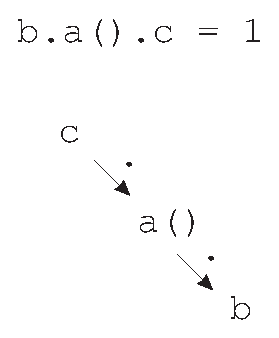
\includegraphics[width=0.25\textwidth]{identuse.eps}
\caption{Parse tree generato per l'espressione \code{b.a().c}}
\label{fig:identuse}
\end{figure}
\\
Come premessa, \`e bene ricordare che il parser del compilatore SMC \`e un parser generato con YACC/Bison, ed \`e quindi un \emph{recursive descendent parser}. Il parse tree generato dal codice di esempio \`e quindi il codice in figura \ref{fig:identuse}.

Ecco come il processo funziona nei vari casi:
\begin{itemize}
\item Se l'identificatore \`e una \textbf{variabile}:
\begin{itemize}
\item se tale variabile si trova in posizione \textbf{iniziale} (cio\`e non ha figli nel parse tree) ,ed \`e una variabile globale o un parametro o una variabile locale (cio\`e se si trova sullo stack), recupero l'indirizzo della variabile e lo metto nel regitro \code{REG\_D}:\\
\code{SET REG\_D, identifier}
\item se tale variabile si trova in posizione \textbf{iniziale} (cio\`e non ha figli nel parse tree), ed \`e una variabile membro della classe corrente bisogna considerare il riferimento \code{this} implicito: l'espressione \emph{expr} deve essere considerata come \code{this.}\emph{expr}.\\
Devo quindi recuperare il riferimento a \code{this} dallo stack e caricarlo nel registro \code{REG\_D}, aggiungendo poi l'offset della variabile come in figura \ref{fig:memberuse}:\\
\code{LEA REG\_D, this;\\
PADD REG\_D, REG\_D, identOffset;}

\begin{figure}[ht]
\centering
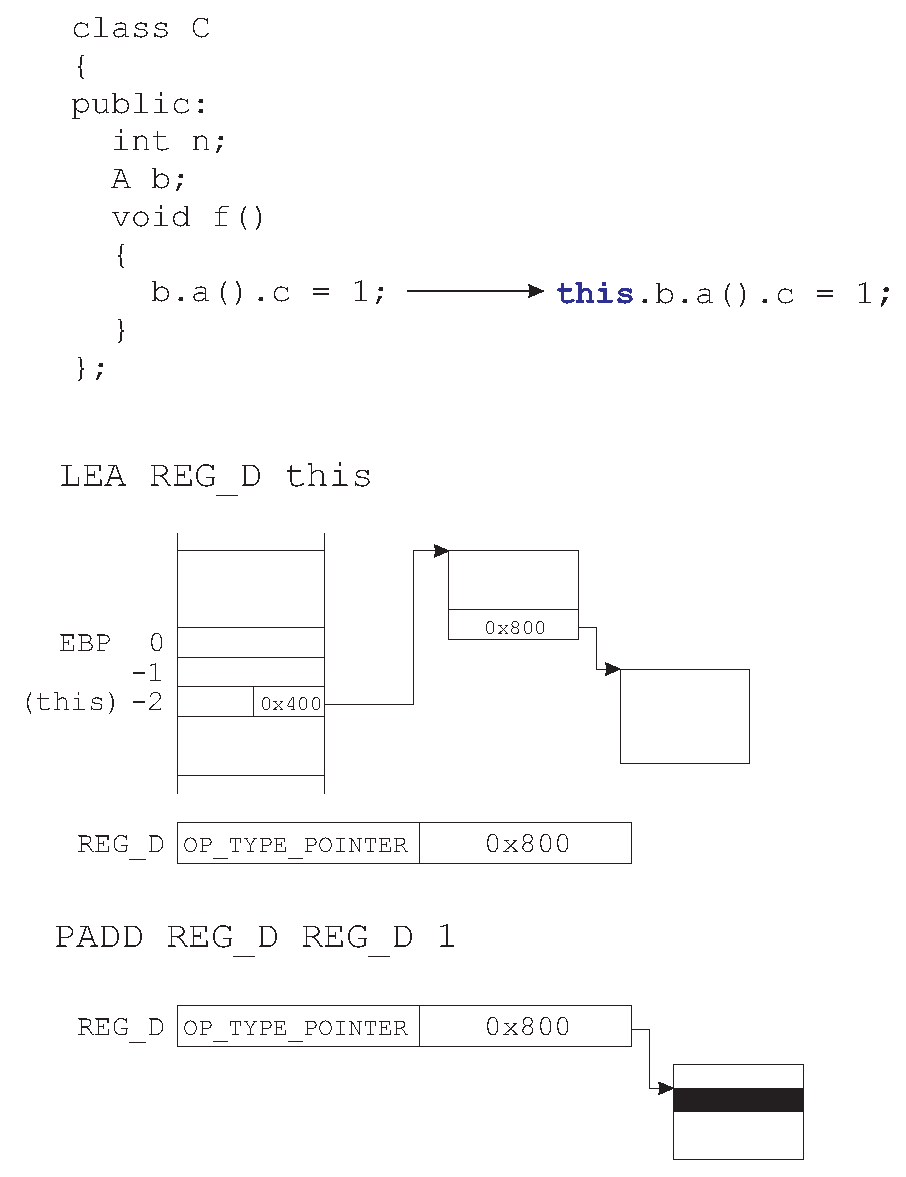
\includegraphics[width=0.75\textwidth]{memberuse.eps}
\caption{Parse tree generato per l'espressione \code{b.a().c}}
\label{fig:memberuse}
\end{figure}

\item se tale variabile si trova in posizione \textbf{intermedia} o \textbf{finale} (cio\`e se ha figli nel parse tree), \`e sicuramente membro di un oggetto: nel registro \code{REG\_D} ricevo gi\`a l'indirizzo base dell'oggetto e ottengo l'indirizzo dell'area dati e quindi del membro specifico con la coppia di istruzioni\\
\code{LEA REG\_D, REG\_D;\\
PADD REG\_D, REG\_D, identOffset;}

\end{itemize}
\item Se l'identificatore \`e una \textbf{funzione} quello che devo fare \`e generare il codice necessario a mettere sullo stack il puntatore a \code{this} corretto per la funzione chiamata, dopodich\'e altri nodi del parse tree si occuperanno di generare il codice necessario a fare il push degli altri parametri e la chiamata a funzione. Anche in questo caso, bisogna distinguere due casi:
\begin{itemize}
\item  se il nodo rappresentante la chiamata nel parse tree non ha figli, si tratta di una chiamata di funzione in prima posizione che pu\`o ritornare un lhs; ad esempio: \code{a().b}.
In questo caso, trattandosi di una chiamata nello scope corrente, quello che il compilatore deve generare \`e il codice necessario a mettere sullo stack un riferimento a \code{this} analogo a quello corrente:\\
\code{CLONE REG\_D, this;\\
PUSH REG\_D;}
\item se il nodo rappresentante la chiamata nel parse tree ha figli, si tratta di una chiamata di funzione con scope; esempio: \code{a.b()}.
In questo caso, il \code{this} all'interno del corpo della funzione \code{b()} \`e proprio un riferimento all'oggetto \code{a}. Poniamo quindi che il codice generato in precedenza porti ad avere un riferimento ad \code{a} nel registro \code{REG\_D}:\\
\code{CLONE REG\_D, REG\_D;\\
PUSH REG\_D;}
\end{itemize}
\end{itemize}




\subsection{Overloading e Overriding}

La ricerca di un simbolo all'interno dello scope corrente \`e piuttosto semplice: \`e sufficiente un cammino all'interno dell'albero di simboli costituente la symbol table, descritto nella sezione \emph{Symbol Table e Type Table}.
Tuttavia, per quanto riguarda le funzioni, la faccenda \`e complicata da un altro fattore: l'overloading.
In caso di pi\`u nomi definiti per una stessa funzione, infatti, il problema \`e diverso: bisogna trovare la funzione ``pi\`u adatta'' per svolgere il compito. Il valore che si calcola per ogni funzione, per capire quanto sia ``adatta'' a essere invocata in un particolare contesto, si dice \emph{fitness value} ed \`e una funzione che prende come input il tipo dei parametri attuali (con i quali la funzione viene chiamata), il tipo dei parametri formali della funzione candidata e una tabella di costi.
L'algoritmo reperisce tutti i record presenti nella \emph{symbol table} aventi lo stesso nome e tipo \code{TYPE\_FUNCTION} e per ognuna di queste funzioni candidate controlla la visibilit\`a nello scope corrente e ne calcola il fitness value usando la seguente procedura:

\noindent
\scriptsize{
\scitef{function}
\scitea{ }
\scitel{BakerDitchfield}
\scitek{(}
\scitea{ }
\scitel{this\_name}
\scitea{ }
\scitek{:}
\scitea{ }
\scitef{name}
\scitek{,}
\scitea{ }
\scitel{args}
\scitea{ }
\scitek{:}
\scitea{ }
\scitel{list}
\scitek{$<$}
\scitea{ }
\scitef{set}
\scitek{$<$}
\scitea{ }
\scitel{tree}
\scitea{ }
\scitek{$>$}
\scitea{ }
\scitek{$>$}
\scitek{)}
\scitea{ } \\
\scitea{{\hspace*{1em}} }
\scitek{:}
\scitea{ }
\scitel{tree\_list}
\scitea{} \\
\scitef{begin}
\scitea{} \\
\scitea{{\hspace*{1em}} }
\scitel{result\_trees}
\scitea{ }
\scitek{:}
\scitea{ }
\scitef{set}
\scitek{$<$}
\scitea{ }
\scitel{tree}
\scitea{ }
\scitek{$>$}
\scitea{ }
\scitek{=}
\scitea{ }
\sciteb{\{\}}
\scitea{} \\
\scitea{{\hspace*{1em}} }
\scitef{for}
\scitea{ }
\scitel{each}
\scitea{ }
\scitel{interpretation}
\scitea{ }
\scitek{(}
\scitel{formals}
\scitek{)}
\scitea{ }
\scitel{corresponding}
\scitea{ }
\scitef{to}
\scitea{ }
\scitel{this\_name}
\scitea{} \\
\scitea{{\hspace*{1em}}{\hspace*{1em}}{\hspace*{1em}} }
\scitef{if}
\scitea{ }
\scitel{formals.length}
\scitea{ }
\scitek{==}
\scitea{ }
\scitel{args.length}
\scitea{ }
\scitef{then}
\scitea{} \\
\scitea{{\hspace*{1em}}{\hspace*{1em}}{\hspace*{1em}}{\hspace*{1em}}{\hspace*{1em}} }
\scitel{new\_tree}
\scitea{ }
\scitek{:}
\scitea{ }
\scitel{tree}
\scitea{} \\
\scitea{{\hspace*{1em}}{\hspace*{1em}}{\hspace*{1em}}{\hspace*{1em}}{\hspace*{1em}} }
\scitel{new\_tree.type}
\scitea{ }
\scitek{=}
\scitea{ }
\scitel{return\_type}
\scitea{} \\
\scitea{{\hspace*{1em}}{\hspace*{1em}}{\hspace*{1em}}{\hspace*{1em}}{\hspace*{1em}} }
\scitel{new\_tree.cost}
\scitea{ }
\scitek{=}
\scitea{ }
\scitee{0}
\scitea{} \\
\scitea{{\hspace*{1em}}{\hspace*{1em}}{\hspace*{1em}}{\hspace*{1em}}{\hspace*{1em}} }
\scitef{for}
\scitea{ }
\scitel{i}
\scitea{ }
\scitek{=}
\scitea{ }
\scitee{1}
\scitea{ }
\scitef{to}
\scitea{ }
\scitel{formals.length}
\scitea{} \\
\scitea{{\hspace*{1em}}{\hspace*{1em}}{\hspace*{1em}}{\hspace*{1em}}{\hspace*{1em}}{\hspace*{1em}}{\hspace*{1em}} }
\scitef{if}
\scitea{ }
\scitel{there}
\scitea{ }
\scitel{exists}
\scitea{ }
\scitel{j}
\scitea{ }
\scitel{in}
\scitea{ }
\scitel{args}
\scitek{[}
\scitel{i}
\scitek{]}
\scitea{ }
\scitel{such}
\scitea{ }
\scitel{that}
\scitea{ }
\scitel{j.type}
\scitea{ }
\scitel{can}
\scitea{ }
\scitel{be}
\scitea{ }
\scitel{converted}
\scitea{ } \\
\scitea{{\hspace*{1em}}{\hspace*{1em}}{\hspace*{1em}}{\hspace*{1em}}{\hspace*{1em}}{\hspace*{1em}}{\hspace*{1em}}{\hspace*{1em}}{\hspace*{1em}} }
\scitef{to}
\scitea{ }
\scitel{formals}
\scitek{[}
\scitel{i}
\scitek{].}
\scitef{type}
\scitea{ }
\scitef{then}
\scitea{} \\
\scitea{{\hspace*{1em}}{\hspace*{1em}}{\hspace*{1em}}{\hspace*{1em}}{\hspace*{1em}}{\hspace*{1em}}{\hspace*{1em}}{\hspace*{1em}}{\hspace*{1em}} }
\scitel{find}
\scitea{ }
\scitel{k}
\scitea{ }
\scitel{in}
\scitea{ }
\scitel{args}
\scitek{[}
\scitel{i}
\scitek{]}
\scitea{ }
\scitel{such}
\scitea{ }
\scitel{that}
\scitea{ }
\scitel{conversion\_cost}
\scitek{(}
\scitel{k.type}
\scitek{,}
\scitea{ } \\
\scitea{{\hspace*{1em}}{\hspace*{1em}}{\hspace*{1em}}{\hspace*{1em}}{\hspace*{1em}}{\hspace*{1em}}{\hspace*{1em}}{\hspace*{1em}}{\hspace*{1em}}{\hspace*{1em}}{\hspace*{1em}} }
\scitel{formals}
\scitek{[}
\scitel{i}
\scitek{].}
\scitef{type}
\scitek{)}
\scitea{ }
\scitek{+}
\scitea{ }
\scitel{k.cost}
\scitea{ }
\scitel{is}
\scitea{ }
\scitel{minimized}
\scitea{} \\
\scitea{{\hspace*{1em}}{\hspace*{1em}}{\hspace*{1em}}{\hspace*{1em}}{\hspace*{1em}}{\hspace*{1em}}{\hspace*{1em}}{\hspace*{1em}}{\hspace*{1em}} }
\scitel{new\_tree.child}
\scitek{[}
\scitel{i}
\scitek{]}
\scitea{ }
\scitek{=}
\scitea{ }
\scitel{k}
\scitea{} \\
\scitea{{\hspace*{1em}}{\hspace*{1em}}{\hspace*{1em}}{\hspace*{1em}}{\hspace*{1em}}{\hspace*{1em}}{\hspace*{1em}}{\hspace*{1em}}{\hspace*{1em}} }
\scitel{new\_tree.cost}
\scitea{ }
\scitek{+=}
\scitea{ }
\scitel{k.cost}
\scitea{} \\
\scitea{{\hspace*{1em}}{\hspace*{1em}}{\hspace*{1em}}{\hspace*{1em}}{\hspace*{1em}}{\hspace*{1em}}{\hspace*{1em}}{\hspace*{1em}}{\hspace*{1em}} }
\scitel{new\_tree.cost}
\scitea{ }
\scitek{+=}
\scitea{ }
\scitel{conversion\_cost}
\scitek{(}
\scitel{k.type}
\scitek{,} \\
\scitea{{\hspace*{1em}}{\hspace*{1em}}{\hspace*{1em}}{\hspace*{1em}}{\hspace*{1em}}{\hspace*{1em}}{\hspace*{1em}}{\hspace*{1em}}{\hspace*{1em}} }
\scitea{}
\scitel{formals}
\scitek{[}
\scitel{i}
\scitek{].}
\scitef{type}
\scitek{)}\\
\scitea{{\hspace*{1em}}{\hspace*{1em}}{\hspace*{1em}}{\hspace*{1em}}{\hspace*{1em}}{\hspace*{1em}}{\hspace*{1em}} }
\scitef{else}
\scitea{} \\
\scitea{{\hspace*{1em}}{\hspace*{1em}}{\hspace*{1em}}{\hspace*{1em}}{\hspace*{1em}}{\hspace*{1em}}{\hspace*{1em}}{\hspace*{1em}}{\hspace*{1em}} }
\scitel{skip}
\scitea{ }
\scitef{to}
\scitea{ }
\scitel{next}
\scitea{ }
\scitel{interpretation}
\scitea{} \\
\scitea{{\hspace*{1em}}{\hspace*{1em}}{\hspace*{1em}}{\hspace*{1em}}{\hspace*{1em}}{\hspace*{1em}}{\hspace*{1em}}{\hspace*{1em}}{\hspace*{1em}} }
\scitek{(}
\scitel{i.e.}
\scitea{ }
\scitel{this}
\scitea{ }
\scitel{interpretation}
\scitea{ }
\scitel{is}
\scitea{ }
\scitel{not}
\scitea{ }
\scitel{consistent}
\scitea{ }
\scitel{with}
\scitea{ }
\scitel{the}
\scitea{ } \\
\scitea{{\hspace*{1em}}{\hspace*{1em}}{\hspace*{1em}}{\hspace*{1em}}{\hspace*{1em}}{\hspace*{1em}}{\hspace*{1em}}{\hspace*{1em}}{\hspace*{1em}} }
\scitel{possible}
\scitea{ }
\scitel{argument}
\scitea{ }
\scitel{types}
\scitek{)}
\scitea{} \\
\scitea{\hspace*{1em}{\hspace*{1em}}{\hspace*{1em}}{\hspace*{1em}}{\hspace*{1em}}{\hspace*{1em}} }
\scitef{end}
\scitea{ }
\scitef{if}
\scitea{} \\
\scitea{{\hspace*{1em}}{\hspace*{1em}}{\hspace*{1em}}{\hspace*{1em}}{\hspace*{1em}} }
\scitef{end}
\scitea{ }
\scitef{for}
\scitea{} \\
\scitea{{\hspace*{1em}}{\hspace*{1em}}{\hspace*{1em}}{\hspace*{1em}}{\hspace*{1em}} }
\scitef{if}
\scitea{ }
\scitel{this}
\scitea{ }
\scitel{interpretation}
\scitea{ }
\scitel{is}
\scitea{ }
\scitel{valid}
\scitea{ }
\scitef{then}
\scitea{} \\
\scitea{{\hspace*{1em}}{\hspace*{1em}}{\hspace*{1em}}{\hspace*{1em}}{\hspace*{1em}}{\hspace*{1em}}{\hspace*{1em}} }
\scitef{if}
\scitea{ }
\scitel{there}
\scitea{ }
\scitel{exists}
\scitea{ }
\scitel{i}
\scitea{ }
\scitel{in}
\scitea{ }
\scitel{result\_trees}
\scitea{ }
\scitel{such}
\scitea{ }
\scitel{that}
\scitea{ }
\scitel{i.type}
\scitea{ }
\scitek{==}
\scitea{ }
\scitel{new\_tree.type}\\
\scitea{{\hspace*{1em}}{\hspace*{1em}}{\hspace*{1em}}{\hspace*{1em}}{\hspace*{1em}}{\hspace*{1em}}{\hspace*{1em}} }
\scitef{then}
\scitea{} \\
\scitea{{\hspace*{1em}}{\hspace*{1em}}{\hspace*{1em}}{\hspace*{1em}}{\hspace*{1em}}{\hspace*{1em}}{\hspace*{1em}}{\hspace*{1em}}{\hspace*{1em}} }
\scitef{if}
\scitea{ }
\scitel{i.cost}
\scitea{ }
\scitek{==}
\scitea{ }
\scitel{new\_tree.cost}
\scitea{ }
\scitef{then}
\scitea{} \\
\scitea{{\hspace*{1em}}{\hspace*{1em}}{\hspace*{1em}}{\hspace*{1em}}{\hspace*{1em}}{\hspace*{1em}}{\hspace*{1em}}{\hspace*{1em}}{\hspace*{1em}}{\hspace*{1em}}{\hspace*{1em}} }
\scitel{i.ambiguous}
\scitea{ }
\scitek{=}
\scitea{ }
\scitef{true}
\scitea{} \\
\scitea{{\hspace*{1em}}{\hspace*{1em}}{\hspace*{1em}}{\hspace*{1em}}{\hspace*{1em}}{\hspace*{1em}}{\hspace*{1em}}{\hspace*{1em}}{\hspace*{1em}} }
\scitef{else}
\scitea{ }
\scitef{if}
\scitea{ }
\scitel{i.cost}
\scitea{ }
\scitek{$<$}
\scitea{ }
\scitel{new\_tree.cost}
\scitea{ }
\scitef{then}
\scitea{} \\
\scitea{{\hspace*{1em}}{\hspace*{1em}}{\hspace*{1em}}{\hspace*{1em}}{\hspace*{1em}}{\hspace*{1em}}{\hspace*{1em}}{\hspace*{1em}}{\hspace*{1em}}{\hspace*{1em}}{\hspace*{1em}} }
\scitel{remove}
\scitea{ }
\scitel{i}
\scitea{ }
\scitel{from}
\scitea{ }
\scitel{result\_trees}
\scitea{} \\
\scitea{{\hspace*{1em}}{\hspace*{1em}}{\hspace*{1em}}{\hspace*{1em}}{\hspace*{1em}}{\hspace*{1em}}{\hspace*{1em}}{\hspace*{1em}}{\hspace*{1em}}{\hspace*{1em}}{\hspace*{1em}} }
\scitel{add}
\scitea{ }
\scitel{new\_tree}
\scitea{ }
\scitef{to}
\scitea{ }
\scitel{result\_trees}
\scitea{} \\
\scitea{{\hspace*{1em}}{\hspace*{1em}}{\hspace*{1em}}{\hspace*{1em}}{\hspace*{1em}}{\hspace*{1em}}{\hspace*{1em}}{\hspace*{1em}}{\hspace*{1em}} }
\scitek{(}
\scitef{else}
\scitea{ }
\scitel{throw}
\scitea{ }
\scitel{away}
\scitea{ }
\scitel{new\_tree}
\scitek{)}
\scitea{} \\
\scitea{\hspace*{1em}{\hspace*{1em}}{\hspace*{1em}}{\hspace*{1em}}{\hspace*{1em}}{\hspace*{1em}}{\hspace*{1em}}{\hspace*{1em}} }
\scitef{end}
\scitea{ }
\scitef{if}
\scitea{} \\
\scitea{{\hspace*{1em}}{\hspace*{1em}}{\hspace*{1em}}{\hspace*{1em}}{\hspace*{1em}}{\hspace*{1em}}{\hspace*{1em}} }
\scitef{else}
\scitea{} \\
\scitea{{\hspace*{1em}}{\hspace*{1em}}{\hspace*{1em}}{\hspace*{1em}}{\hspace*{1em}}{\hspace*{1em}}{\hspace*{1em}}{\hspace*{1em}}{\hspace*{1em}} }
\scitel{add}
\scitea{ }
\scitel{new\_tree}
\scitea{ }
\scitef{to}
\scitea{ }
\scitel{result\_trees}
\scitea{} \\
\scitea{\hspace*{1em}{\hspace*{1em}}{\hspace*{1em}}{\hspace*{1em}}{\hspace*{1em}}{\hspace*{1em}} }
\scitef{end}
\scitea{ }
\scitef{if}
\scitea{} \\
\scitea{{\hspace*{1em}}{\hspace*{1em}}{\hspace*{1em}}{\hspace*{1em}}{\hspace*{1em}} }
\scitef{end}
\scitea{ }
\scitef{if}
\scitea{} \\
\scitea{{\hspace*{1em}}{\hspace*{1em}}{\hspace*{1em}} }
\scitef{end}
\scitea{ }
\scitef{if}
\scitea{} \\
\scitea{{\hspace*{1em}} }
\scitef{end}
\scitea{ }
\scitef{for}
\scitea{} \\
\scitea{{\hspace*{1em}} }
\scitef{for}
\scitea{ }
\scitel{each}
\scitea{ }
\scitel{tree}
\scitea{ }
\scitel{in}
\scitea{ }
\scitel{result\_trees}
\scitea{} \\
\scitea{{\hspace*{1em}}{\hspace*{1em}}{\hspace*{1em}} }
\scitef{if}
\scitea{ }
\scitel{tree.ambiguous}
\scitea{ }
\scitef{then}
\scitea{} \\
\scitea{{\hspace*{1em}}{\hspace*{1em}}{\hspace*{1em}}{\hspace*{1em}}{\hspace*{1em}} }
\scitel{remove}
\scitea{ }
\scitel{tree}
\scitea{ }
\scitel{from}
\scitea{ }
\scitel{result\_trees}
\scitea{} \\
\scitea{{\hspace*{1em}}{\hspace*{1em}}{\hspace*{1em}} }
\scitef{end}
\scitea{ }
\scitef{if}
\scitea{} \\
\scitea{{\hspace*{1em}} }
\scitef{end}
\scitea{ }
\scitef{if}
\scitea{} \\
\scitea{{\hspace*{1em}} }
\scitel{return}
\scitea{ }
\scitel{result\_trees}
\scitea{} \\
\scitef{end}
\scitea{} \\
\scitea{}
} %end tiny
\normalfont
\normalsize
\\
Se pi\`u di una funzione ha lo stesso fitness value, viene generato un errore.

Ancora diverso \`e il caso di \emph{function overriding}: in questa situazione, una funzione viene nascosta da una funzione con nome \textbf{e} parametri identici. Questa situazione si verifica quando ridefiniamo una funzione presente in una classe base nella classe derivata; per esempio:

%esempio3.cpp
\noindent
\scriptsize{
\scitef{class}
\scitea{ }
\scitel{A}
\scitea{ }
\scitek{\{}
\scitea{} \\
\scitef{public}
\scitek{:}
\scitea{} \\
\scitea{{\hspace*{1em}} }
\scitef{void}
\scitea{ }
\scitel{f}
\scitek{()}
\scitea{ } 
\scitek{\{}
\scitea{  } 
\scitek{...}
\scitea{ } 
\scitek{\}}\\
\scitek{\};}
\scitea{} \\
\scitea{} \\
\scitef{class}
\scitea{ }
\scitel{B}
\scitea{ }
\scitek{:}
\scitea{ }
\scitef{public}
\scitea{ }
\scitel{A}
\scitea{ } 
\scitek{\{}
\scitea{} \\
\scitef{public}
\scitek{:}
\scitea{} \\
\scitea{{\hspace*{1em}} }
\scitef{void}
\scitea{ }
\scitel{f}
\scitek{()}
\scitea{ }
\scitek{\{}
\scitea{ }
\scitek{...}
\scitea{ }
\scitek{\}}
\scitea{{\hspace*{1em}} } \\
\scitea{{\hspace*{1em}} }
\scitef{void}
\scitea{ }
\scitel{g}
\scitek{()}
\scitea{ } 
\scitek{\{}
\scitea{ } 
\scitel{f}
\scitek{();}
\scitea{ } 
\scitec{/*B::f() hides A::f()*/}
\scitea{ }
\scitek{\}}
\scitea{} \\
\scitek{\};}
\scitea{} \\
\scitea{}
}
\normalfont
\normalsize

Nel caso in cui siano coinvolte funzioni virtuali, vengono innescati meccanismi pi\`u complessi per produrre un comportamento corretto. Questi meccanismi sono discussi nella sezione seguente.

\subsection{Chiamate a funzione virtuale: polimorfismo}

Se si fa l'\emph{overriding} di una funzione normale, quello che si ottiene quando si chiama tale funzione \`e una chiamata a funzione con binding statico. In pratica, compilando con SMC il seguente programma, l'output che si ottiene \`e ``Instrument::play''
\\
Esempio: Instrument
\\
\noindent
\scriptsize{
\scitej{\#include "output.hs"} \\
\scitef{class}
\scitea{ }
\scitel{Instrument}
\scitea{ } \\
\scitek{\{}
\scitea{} \\
\scitef{public}
\scitek{:}
\scitea{} \\
\scitea{{\hspace*{1em}} }
\scitef{void}
\scitea{ }
\scitel{play}
\scitek{()}
\scitea{ } \\
\scitea{{\hspace*{1em}} }
\scitek{\{}
\scitea{} \\
\scitea{{\hspace*{1em}}{\hspace*{1em}}{\hspace*{1em}} }
\scitel{print}
\scitek{(}
\sciteg{"Instrument::play"}
\scitek{);}
\scitea{} \\
\scitea{{\hspace*{1em}} }
\scitek{\}}
\scitea{} \\
\scitek{\};}
\scitea{} \\
\scitea{} \\
\scitec{// Wind objects are Instruments} \\
\scitec{// because they have the same interface:} \\
\scitef{class}
\scitea{ }
\scitel{Wind}
\scitea{ }
\scitek{:}
\scitea{ }
\scitel{Instrument}
\scitea{ } \\
\scitek{\{}
\scitea{} \\
\scitef{public}
\scitek{:}
\scitea{} \\
\scitea{{\hspace*{1em}} }
\scitec{// Redefine interface function:} \\
\scitea{{\hspace*{1em}} }
\scitef{void}
\scitea{ }
\scitel{play}
\scitek{()}
\scitea{} \\
\scitea{{\hspace*{1em}} }
\scitek{\{}
\scitea{} \\
\scitea{{\hspace*{1em}}{\hspace*{1em}}{\hspace*{1em}} }
\scitel{print}
\scitek{(}
\sciteg{"Wind::play"}
\scitek{);}
\scitea{} \\
\scitea{{\hspace*{1em}} }
\scitek{\}}
\scitea{} \\
\scitek{\};}
\scitea{} \\
\scitea{} \\
\scitef{void}
\scitea{ }
\scitel{tune}
\scitek{(}
\scitel{Instrument}
\scitea{ }
\scitek{\&}
\scitea{ }
\scitel{i}
\scitek{)}
\scitea{ } \\
\scitek{\{}
\scitea{} \\
\scitea{{\hspace*{1em}} }
\scitel{i}
\scitek{.}
\scitel{play}
\scitek{();}
\scitea{} \\
\scitek{\}}
\scitea{} \\
\scitea{} \\
\scitef{int}
\scitea{ }
\scitel{main}
\scitek{()}
\scitea{ } \\
\scitek{\{}
\scitea{} \\
\scitea{{\hspace*{1em}} }
\scitel{Wind}
\scitea{ }
\scitel{flute}
\scitek{;}
\scitea{} \\
\scitea{{\hspace*{1em}} }
\scitel{tune}
\scitek{(}
\scitel{flute}
\scitek{);}
\scitea{ }
\scitec{// Upcasting} \\
\scitea{{\hspace*{1em}} } \\
\scitea{{\hspace*{1em}} }
\scitef{return}
\scitea{ }
\scitee{0}
\scitek{;}
\scitea{} \\
\scitek{\}}
\scitea{} \\
\scitea{} \\
\scitea{} \\
\scitea{}
} %end tiny
\normalfont
\normalsize

Ma se si aggiunge la keyword \textbf{virtual} davanti al metodo \emph{Instrument::play}, il comportamento cambia: l'output \`e ``Wind::play'' grazie al fatto che la keyword virtual dice al compilatore che c'\`e bisogno di un comportamento \emph{polimorfo} e di usare quindi il binding dinamico. La funzione da chiamare \`e decisa a run-time in modo efficiente tramite l'istruzione assembly VCALL e la cosiddetta v-table, la tabella delle funzioni virtuali collegata ad ogni oggetto.
Vediamo come funziona tutto il meccanismo, cosa succede in fase di compilazione e cosa in fase di esecuzione.

\subsubsection{Fase di compilazione}

In fase di compilazione, durante la dichiarazione di una funzione virtuale \emph{f} come membro di una classe \textbf{A}, il compilatore esegue le seguenti operazioni:

\begin{itemize}
\item[-] come nel caso di funzioni non virtuali, il compilatore costruisce il simbolo per la funzione \emph{f} (oggetto SymDef);
\item[-] se la funzione \emph{f} \`e la prima ad essere dichiarata come virtuale per la classe \textbf{A}, il compilatore costruisce la v-table per tale classe. La v-table, tabella delle funzioni virtuali, \`e un array di simboli (oggetti SymDef) che viene associato alla classe di cui la funzione \`e membro;
\item[-] il simbolo della funzione \emph{f} viene aggiunto alla v-table: ci sono ora due ulteriori possibilit\`a:
\begin{itemize}
\item non siamo in presenza di un \emph{override}: nessun simbolo per \emph{f} \`e gi\`a stato definito in una classe antenata di \textbf{A} (oppure \textbf{A} \`e alla base della gerarchia):\\
alla v-table di \textbf{A} viene aggiunto un nuovo record con il simbolo per \emph{f};\\
al campo \code{virtualIndex} del simbolo viene assegnato l'indice di questo nuovo record;

\item siamo in presenza di un \emph{override}, e il simbolo per \emph{f}  definito in precedenza \`e anch'esso dichiarato come \textbf{virtual}:\\
nella v-table di \textbf{A} viene reperito l'indice del precedente simbolo per \emph{f};\\
a questa posizione viene inserito il nuovo simbolo per \emph{f} sovrascrivendo il vecchio.\\
\end{itemize}
\end{itemize}
Affinch\'e le v-table siano costruite correttamente \`e inoltre necessario che quando viene dichiarata una nuova classe \textbf{B} derivata da una classe precedente \textbf{A}, se \textbf{A} ha una v-table, questa sia copiata identica in \textbf{B}.\\
I passi di questo algoritmo sono riassunti ed esemplificati nella figura\ref{fig:virtual}.

\begin{figure}[ht]
\centering
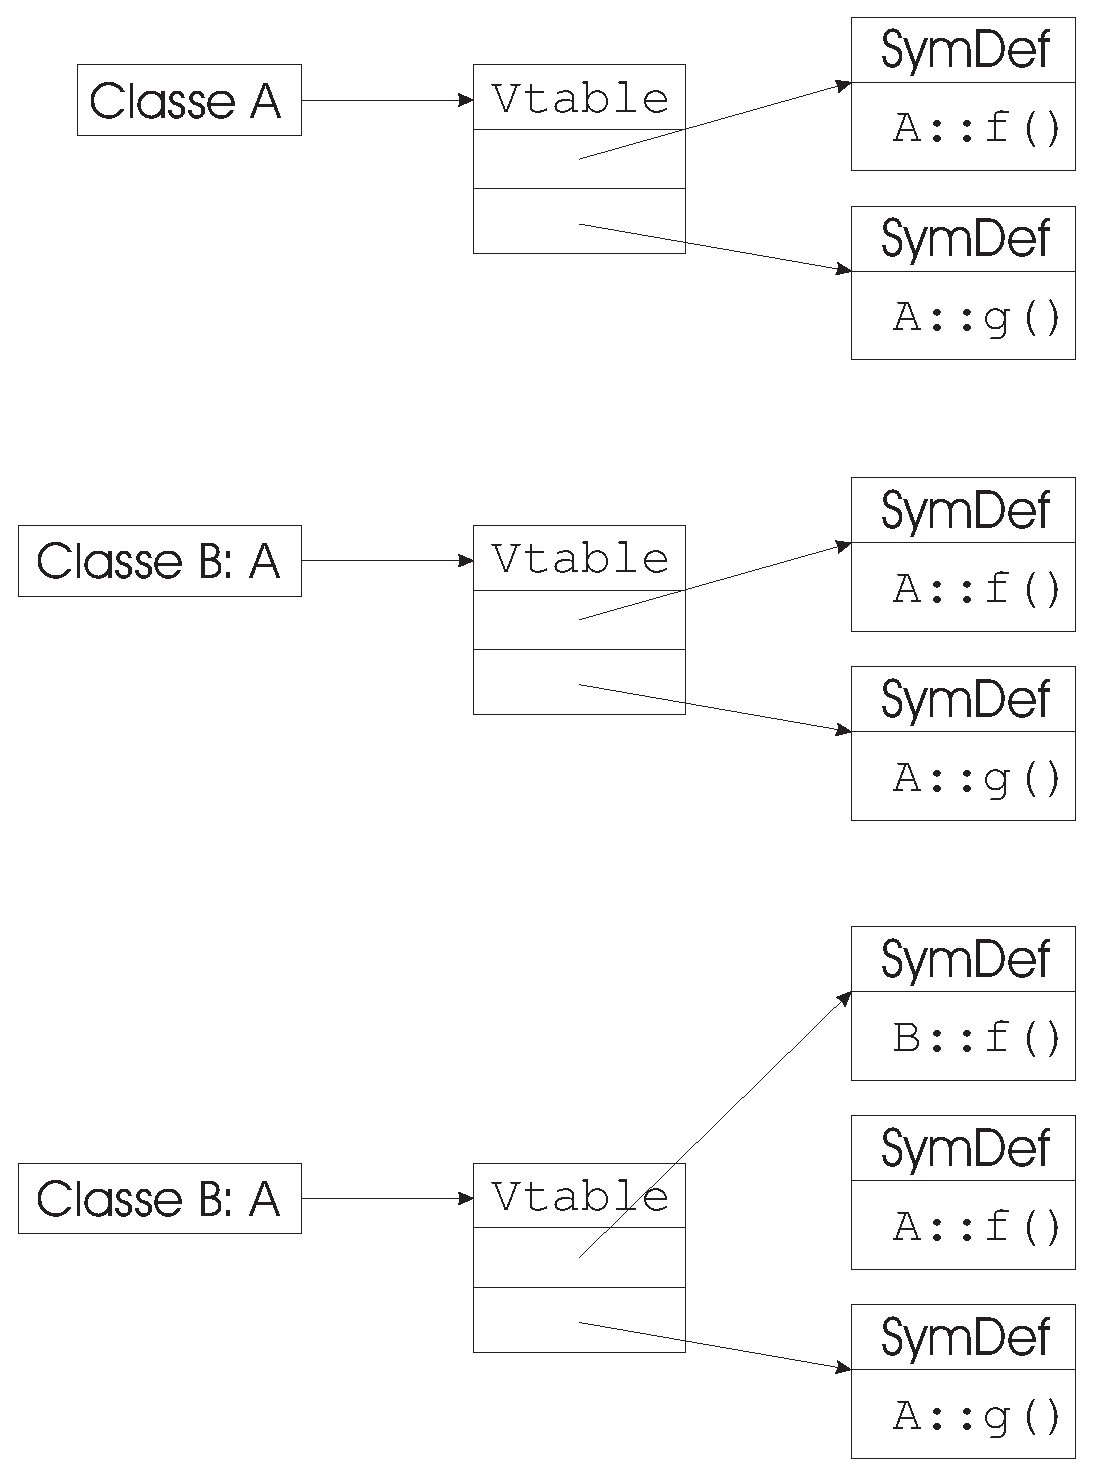
\includegraphics[width=0.6\textwidth]{virtual.eps}
\caption{Dichiarazione di funzioni virtuali: in alto la v-table di \textbf{A} con due funzioni virtuali, \emph{f} e \emph{g}, al centro la v-table di \textbf{B} subito dopo la dichiarazione della classe, in basso la v-table di \textbf{B} dopo l'overriding della funzione virtuale \emph{f}}
\label{fig:virtual}
\end{figure}

Durante la chiamata a funzione, il compilatore vede se la funzione chiamata \`e virtuale o meno, e in tal caso genera un'istruzione \code{VCALL virtual\_function\_index} al posto di una canonica \code{CALL object\_id function\_index}. Il perch\'e non sia necessario l'object\_id nel caso di una chiamata virtuale sar\`a chiaro in seguito, quando analizzeremo il comportamento in fase di esecuzione.

Infine, durante la generazione del codice eseguibile, il compilatore scrive dopo l'header dell'eseguibile e la string table un'ulteriore tabella, detta object table. Tale tabella contiene informazioni su tutte le classi presenti nel programma generato; tra queste informazioni ci sono l'offset all'interno della sezione di codice eseguibile di tutte le funzioni della classe e la sua v-table.

\subsubsection{Fase di esecuzione}

Per capire meglio cosa accade in fase di esecuzione, vediamo il codice generato dal compilatore per il programma di esempio Instrument, con dichiarazione di funzione normale e con dichiarazione di funzione virtuale:\\
\newline
Chiamata normale
 \\
\scriptsize{
\texttt{
27:	PUSH REG\_D \\
28:	CALL object no:3338408 func \#0
}}
\normalsize
\\
\newline
Chiamata virtuale
\\
\scriptsize{
\texttt{
27:	PUSH REG\_D \\
28:	VCALL func \#0
}}
\normalsize
\newline

Come descritto nella sezione ``Il linguaggio assembly'', nella macchina virtuale per SMC ogni tipo di dato \`e incapsulato in un Operand, che contiene il valore e un tag per identificare il tipo del dato correntemente ospitato nella struttura. 

\begin{figure}[ht]
\centering
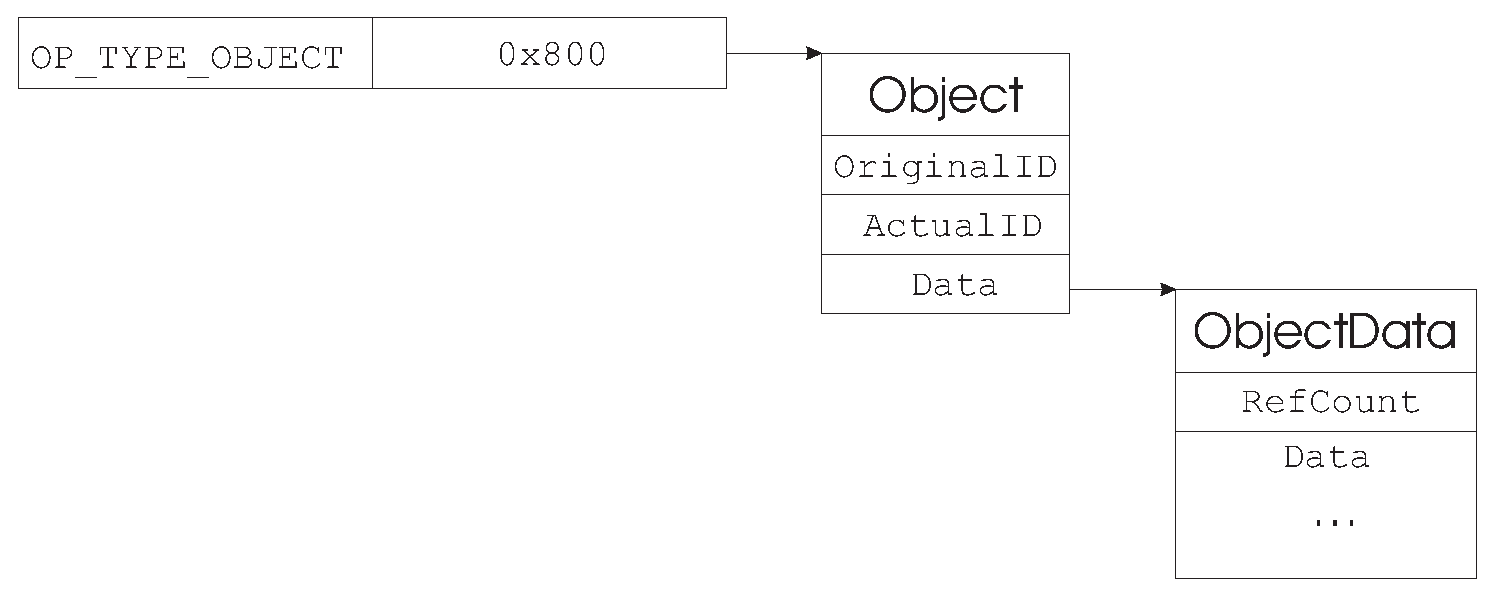
\includegraphics[width=0.8\textwidth]{object.eps}
\caption{Qualsiasi oggetto viene rappresentato nella memoria della VM in questo modo. La grandezza della sezione \code{Data} dipende dalla dimensione dell'oggetto}
\label{fig:object}
\end{figure}

Nel caso in questione, il registro D della macchina virtuale contiene un tipo di dato \code{OP\_TYPE\_OBJECT}: il parametro \textbf{this} per la funzione chiamata.
Al tipo di dato \code{OP\_TYPE\_OBJECT} corrisponde la struttura descritta in figura \ref{fig:object}
I campi OriginalID e ActualID contengono l'ID univoco della class a partire dalla quale \`e stato creato l'oggetto. In particolare il campo OriginalID non viene mai modificato; in questo modo anche se passo l'oggetto tramite un riferimento alla classe base, come accade nell'esempio, la VCALL sa sempre qual'\`e la classe originale.
\begin{figure}[ht]
\centering
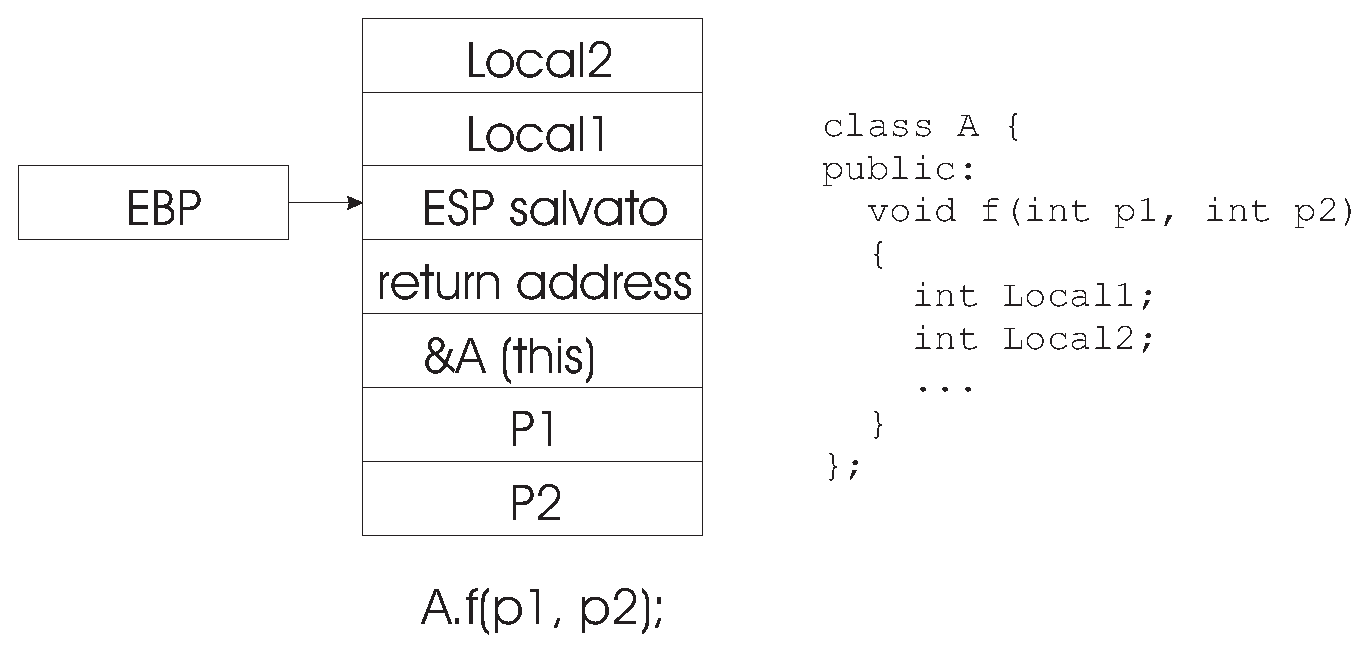
\includegraphics[width=0.8\textwidth]{stack.eps}
\caption{La configurazione dello stack al momento dell'esecuzione della prima istriuzione della funzione}
\label{fig:stack}
\end{figure}
\\
Quindi nel momento in cui si esegue una chiamata a funzione il puntatore a \textbf{this} \`e sempre presente sullo stack in posizione prefissata; un esempio di configurtazione dello stack al momento della 
chiamata \`e rappresentata in figura~\ref{fig:stack}.
\\
I passi di una chiamata virtuale si riassumono quindi ai seguenti (figura~\ref{fig:vcall}):

\begin{figure}[ht]
\centering
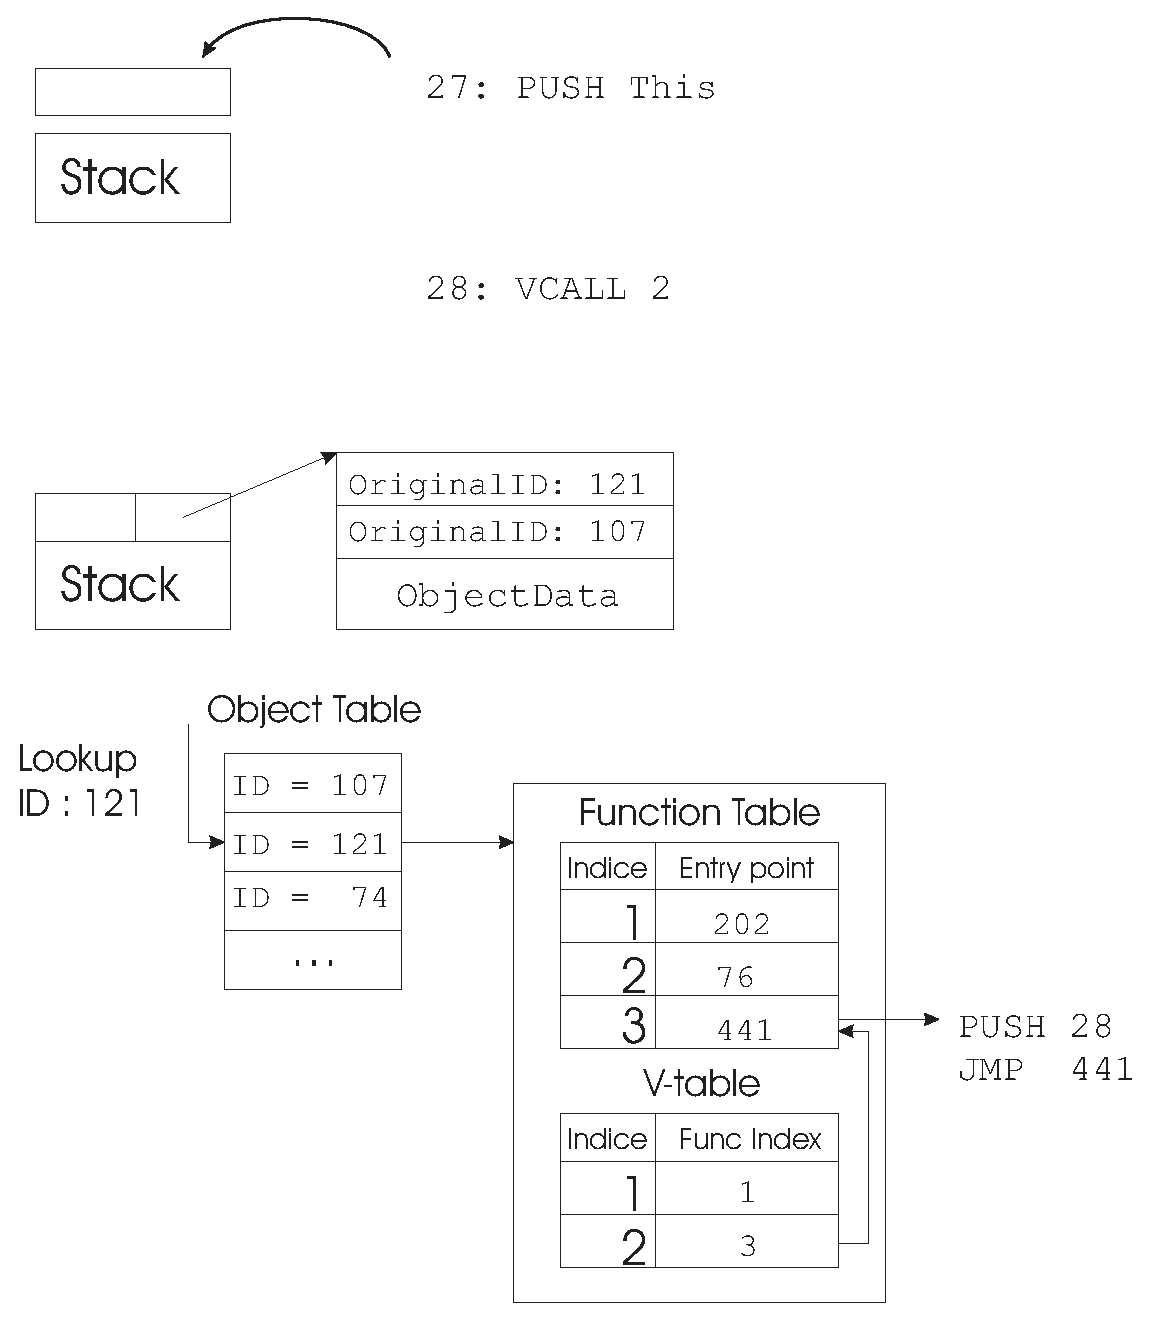
\includegraphics[width=0.8\textwidth]{vcall.eps}
\caption{Una chiamata a funzione virtuale: usando il parametro implicito This messo sullo stack, 
si ricava l'ID della classe originale dell'oggetto, e da questo tutte le informazioni necessarie alla chiamata della funzione.}
\label{fig:vcall}
\end{figure}


\begin{itemize}
\item reperimento di \textbf{this} sullo stack;
\item da questo, otteniamo l'OriginalID dell'oggetto;
\item usiamo l'ID come chiave per trovare le informazioni sulla classe corrispondente nella Object Table;
\item tra queste vi sono la v-table e le l'entry point di tutte le funzioni definite in quella casse;
\item con queste informazioni e il virtualIndex, l'operando della VCALL, si reperisce l'entry point corretto;
\item si esegue un salto incondizionato a questo indirizzo, salvando il return address sullo stack.
\end{itemize}

Per quanto riguarda una chiamata a funzione standard, il procedimento \`e pi\`u semplice e pi\`u veloce: l'ID della classe \`e gi\`a noto al tempo di compilazione ed \`e quindi inserito come primo operando dell'istruzione CALL. Inoltre l'indice della funzione, specificato come secondo operando, non \`e un indice per la v-table, ma direttamente un indice per la Function Table di quella classe.

\appendix
\section{Appendice: gli esempi}

Di seguito sono elencati e brevemente illustrati gli esempi forniti a corredo

\begin{center}
\begin{tabular}{l|p{5.5 cm}}
\hline
\textbf{Nome} & \textbf{Descrizione}\\
\hline
\code{array.cs} & illustra l'utilizzo degli array e il passaggio di questi a una funzione.\\
\code{instrument1.cs} & esempio ereditariet\`a: no polimorfismo.\\
\code{instrument2.cs} & esempio ereditariet\`a: polimorfismo con funzioni virtuali.\\
\code{instrument3.cs} & esempio ereditariet\`a a pi\`u livelli con polimorfismo.\\
\code{ObjectObject.cs} & oggetti membro di oggetti, funzioni che ritornano riferimenti a oggetti membro.\\
\code{perlin.cs} & generatore di perlin noise: test delle principali capacit\`a aritmetiche del linguaggio e della VM, test sulle chiamate native.\\
\code{prova1.cs} & semplice test di scope sulle variabili.\\
\code{string.cs} & test sulle stringhe.\\
\code{switch.cs} & test del costrutto switch.\\
\code{while.cs} & test del costrutto while.\\
\hline
\end{tabular}
\end{center}

\section{Appendice: sorgenti di ispirazione}

Molti libri mi hanno ispirato nel design del linguaggio: in particolare \cite{GS03} per la struttura della VM, \cite{Rob00} per come accedere ai mebri di una classe in linguaggio assembly, \cite{Bruce02} per l'implementazione e il funzionamento delle chiamate virtuali e \cite{Bjarne} per la grammatica di un lingueggio con classi.


\bibliographystyle{abbrv}
\bibliography{biblio}


\end{document}
